\chapter{Results}\label{chap:results}
% -------------------------
%% QUOTE
\vspace*{\fill}
\epigraph{If you're doing an experiment, you should report everything that you think might make it invalid — not only what you think is right about it; other causes that could possibly explain your results; and things you thought of th||you've eliminated by some other experiment, and how they worked — to make sure the other fellow can tell they have been eliminated.}%
{\textit{Surely You're Joking, Mr. Feynman!, p. 341}\\ \textsc{Richard Feynman}}
\clearpage{\thispagestyle{empty}\cleardoublepage}
%%
%% Body of the chapter
%%%%%%%%%%%%%%%%%%%%%%

In this chapter, the results from every experiment is presented in the same order as chapter \ref{chap:experimental}. 

\section{PEC nanogels}
\subsection{Gels with \ce{Cr^{3+}} as crosslinker}

\index{\ce{Cr^3+}} Table \ref{tab:crGelsAt} shows the lowest concentration for gel formation for the different polymers used in the experiments. As seen the table, gel was only formed with Alcoflood 254 S for the highest concentration tested, namely 2 wt. \%. However, it is possible that gels could have been formed at lower concentrations in the interval between 1 wt. \% and 2 wt. \%. Alcomer 24 UK formed gel at 0.5 wt. \% but not at 0.25 wt. \%. It is possible that the highest molecular weight polymer Flopaam 5115 VHM could have formed gels at concentrations lower than 0.5 wt. \%.

\begin{table}[h]
\small
\centering
\caption{Minimum concentration for gel formation for the different polymers}
\label{tab:crGelsAt}
\begin{tabular}{c c c c >{\columncolor[gray]{0.8}}c } 
\toprule
\textbf{Name} & \textbf{Producer} & \textbf{MW} & \textbf{Concentration} & \textbf{Will gel at} \\ 
&& [MDa] & [wt\%] & [wt\%]  \\
\midrule 
Alcoflood 254 S     & BASF    & 0.5 & 0.5, 1.0 and 2.0 & 2\\
Alcomer 24 UK       & BASF    & 6 & 0.25, 0.5, 1.0 and 2.0 & $\geq 0.5$ \\ 
Flopaam 5115 VHM    & SNF Floerger    & 12+ & 0.5, 1.0 and 2.0 & $\geq 0.5$ \\ 
\bottomrule
\end{tabular}
\end{table}

In order to obtain data for testing of the simulator \--- developed for transport of nanoparticles and polymer, and with a functionality of time delayed gel formation (see Chapter \ref{chap:simulation})\--- some gel formation experiments were conducted where the polymer concentration was varied from 0.25 wt. \% to 1 wt. \% and the concentration of \ce{Cr^{3+}} was varied from 22 ppm to 113 ppm. For this series of experiments, Alcomer 24 UK was used as polymer. For concentrations higher than 22 ppm, the polymer viscosity was apparently not dependent on the cross-binder concentration (within the accuracy of the measured viscosities as discussed before). The viscosities of the solutions were measured directly after preparation and after one day of aging. Figure \ref{cht:viscAlco} shows viscosity as function of shear rate for three polymer concentrations. 
\begin{figure}
    \centering
    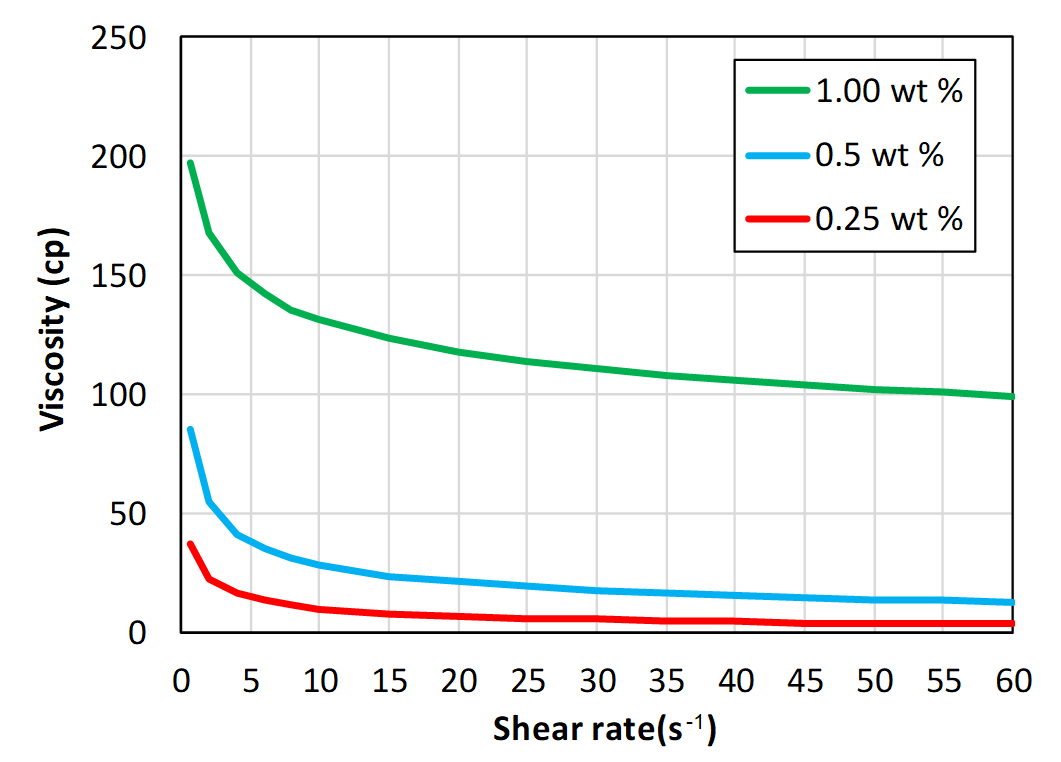
\includegraphics[width=.75\textwidth]{img/cht/viscAlcomer.png}
    \caption{Viscosity as function of shear rate and polymer concentration for Alcomer 24 UK}
    \label{cht:viscAlco}
\end{figure}

Figure \ref{cht:viscPolcModel} shows an example of a reaction model designed based on viscosities measured at a shear rate of 12.7 s$^-1$ for the fresh made solutions and after one day of aging. The blue curve corresponds to the polymer which has not reacted, i.e. data taken from Figure \ref{cht:viscAlco}. It also corresponds to the viscosities for aging times less than 50 days with reference to Figure \ref{cht:jennTai} (although some viscosity increase was seen in this period). The red curve corresponds to maximum viscosities for the solutions, corresponding to the value after 60 days in Figure \ref{cht:jennTai} that is only valid for a single polymer concentration. The green curve is for aging time laying between no gelling and complete gelling. Again, with reference to Figure \ref{cht:jennTai} the green curve would be valid for an aging time of 55 days. In the reaction model, it is assumed that the viscosity increases linearly with time in the gelling period. Again, as mentioned above, the reaction model was solely made to have some reality based data to be used for testing of the simulator model. 

\begin{figure}
    \centering
    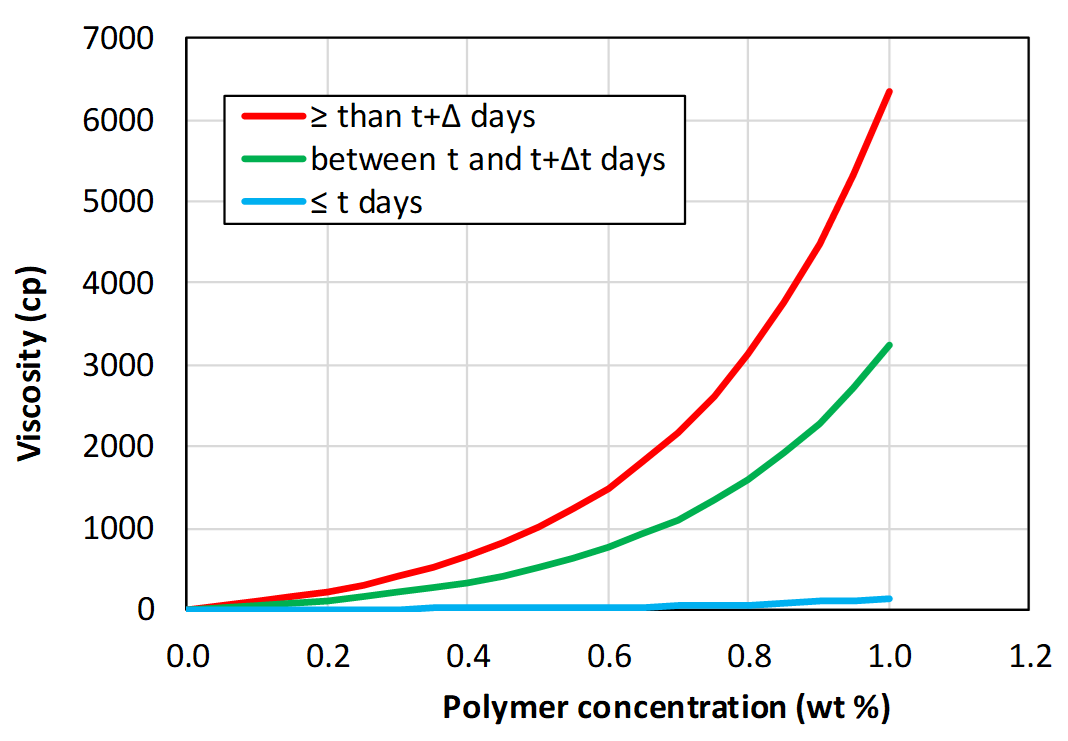
\includegraphics[width=.75\textwidth]{img/cht/viscPolcModel.png}
    \caption{Reaction model for Alcomer 24 UK}
    \label{cht:viscPolcModel}
\end{figure}




\subsection{Polyelectrolyte complexes according to the Texas A\&M recipe}

\index{polyelectrolyte complexes} Figure \ref{cht:s10visc50} shows viscosity as function of time on logarithmic and linear scales. As shown in the figure, there were only minor increases in viscosity the first 7 days. After 23 days, the viscosity was increased significantly and it increased further when the last sample was measured after 37 days. Simple power functions were fitted to the experimental data. The plot on linear scale suggest that the largest effect of the cross binding occurred after approximately 20 days. 

\begin{figure}
    \centering
    \makebox[\textwidth][c]{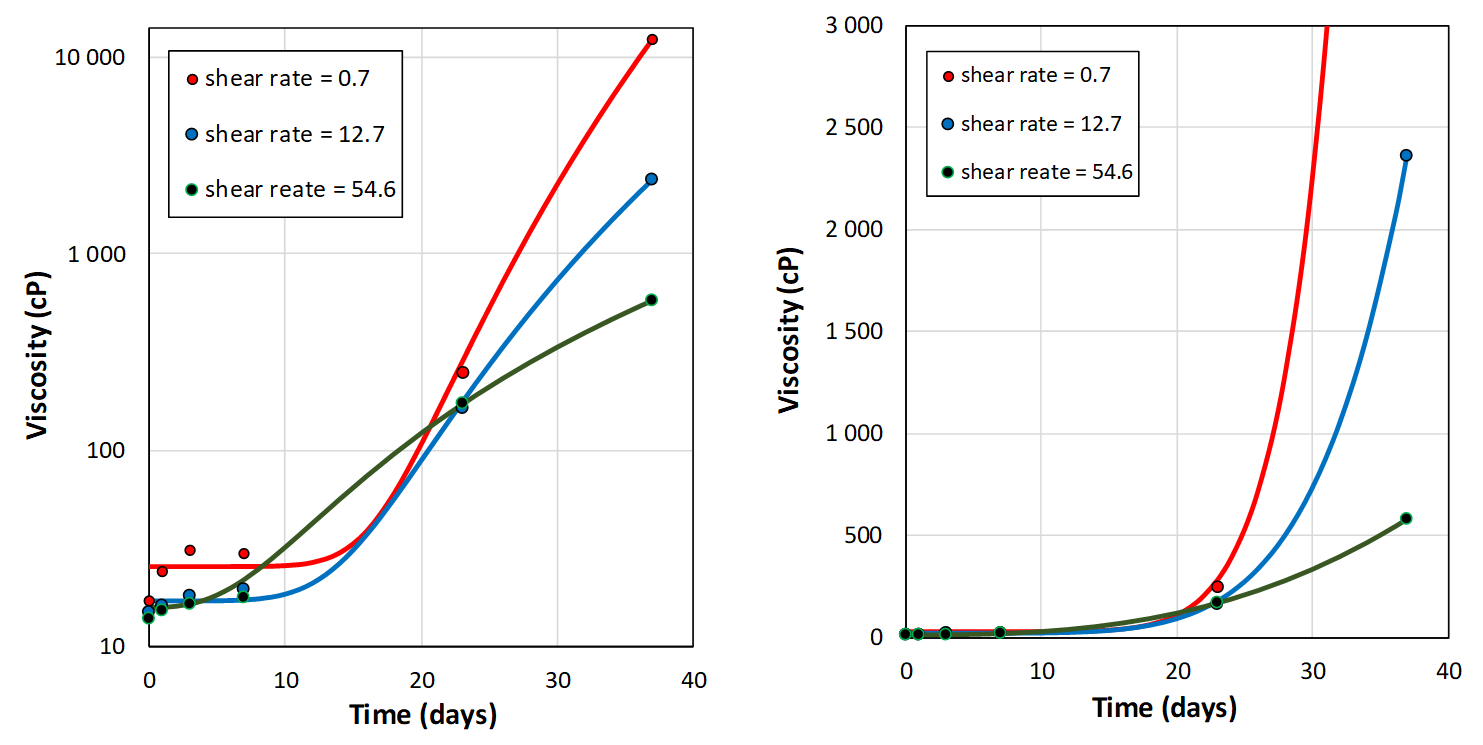
\includegraphics[width=1.2\textwidth]{img/cht/s10visc50.png}}
    \caption{Viscosity as function of aging time for Series 10 samples aged at 50~\celsius~ on logarithmic (left) and linear (right) scales}
    \label{cht:s10visc50}
\end{figure}

Figure \ref{cht:s3536visc} shows the results from viscosity measurements on Series 35 (polymer/PEC solutions made using 0.498 wt. \% of Alcomer 24 UK) and Series 36  0.490 wt. \% of Flopaam 5115 VHM). As seen in Figure \ref{cht:s3536visc}, the viscosity increased quickly, and gels were formed in the vials (visual observations) already after 3 days of aging. The apparent decrease in viscosity at longer aging times are artifacts due to the measurement method as the solutions still appeared as gels.

\begin{figure}
    \centering
    \makebox[\textwidth][c]{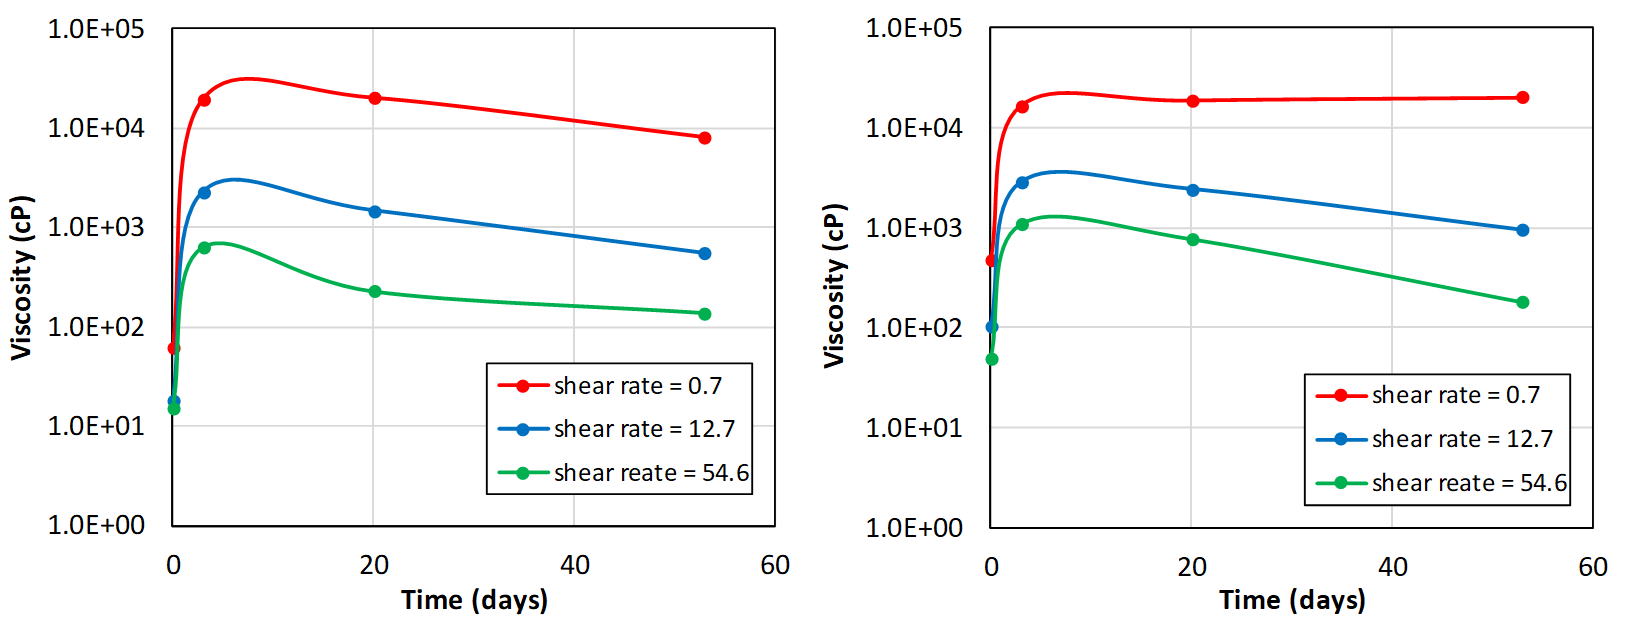
\includegraphics[width=1.2\textwidth]{img/cht/s3536.png}}%
    \caption{Viscosity as function of aging time for Series 35 samples (left) and Series 36 samples (right), aged at 80~\celsius}
    \label{cht:s3536visc}
\end{figure}

Two more systems were made in an equivalent manner using Alcomer 24 UK, but with reduced concentrations of \ce{Cr^{3+}} (60 ppm in Series 42 and 41 ppm in Series 47). Both systems gelled after 3 days of aging at 80~\celsius.

\subsection{Polyelectrolyte complexes based on amine POSS}
\index{amine POSS} Figure \ref{cht:s17visc80} compares the viscosities of the four solutions in this category at 80~\celsius~(their composition is summarized in Table \ref{tab:polyPecComp}).

\begin{figure}
    \centering
    \makebox[\textwidth][c]{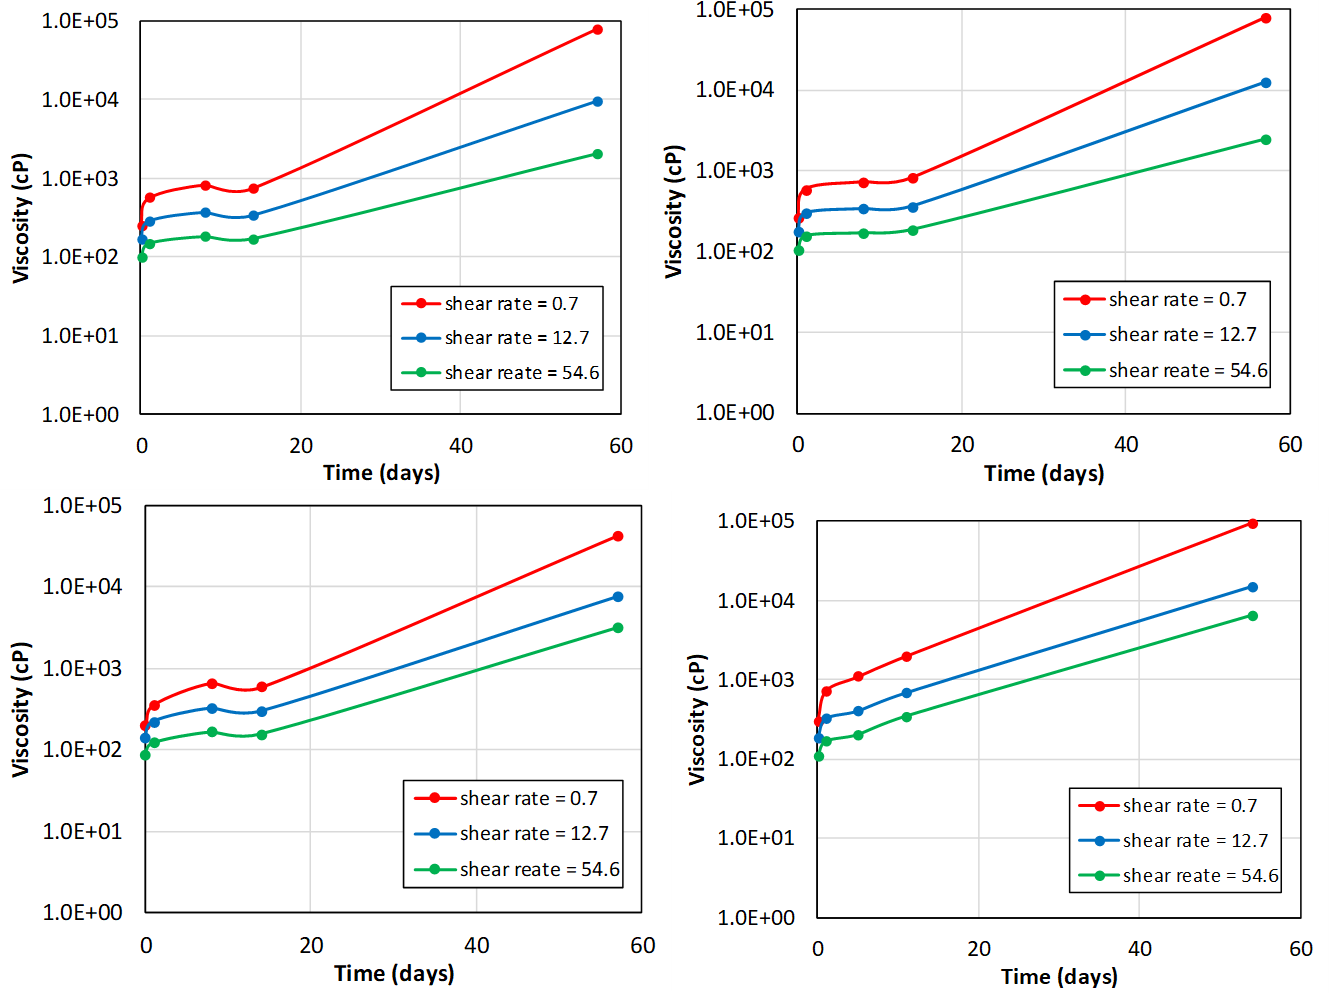
\includegraphics[width=1.2\textwidth]{img/cht/s17visc80.png}}
    \caption{Polymer/PEC solutions aged at 80~\celsius. Upper left: Series 17 samples. Upper right: Series 18 samples. Lower left: Series 19 samples. Lower right: Series 20 samples.}
    \label{cht:s17visc80}
\end{figure}

The figure shows that on the first day of aging, the viscosities in all solutions increased to some degree. Then all three solutions with PEC (Series 17 through 19) exhibited an almost constant viscosity for 14 days. After 57 days, a significant increases in viscosity was seen for all the three solutions. Due to summer holidays, there was no measurements taken between days 14 and 57, and it is not possible to know the exact length of the "constant viscosity period". After 14 days the samples in Series 17 through Series 19 were characterized as viscous fluids. The samples in Series 20 were prepared without PVS and thus without PEC. For this series, the solution was characterized as viscous fluid after 5 days and as week gel after 11 days. Comparison of the samples made with and without PEC shows that incorporation of the amine POSS in PEC reduced gel formation significantly. Surprisingly, no effect was observed by increasing the amount of PVS.

A solution made with Flopaam 5115 VHS and PEC (Series 38) is compared with the same polymer, gelled with \ce{Cr^{3+}} as cross binder (101 ppm, Series 1) in Figure \ref{cht:s38visc80}. The polymer concentration was 1.00 wt.\% and the concentrations of amine POSS and PVS were similar to those of Series 17. Series 38 was aged at 80~\celsius~whereas Series 1 was aged at 50~\celsius.

\begin{figure}[h]
    \centering
    \makebox[\textwidth][c]{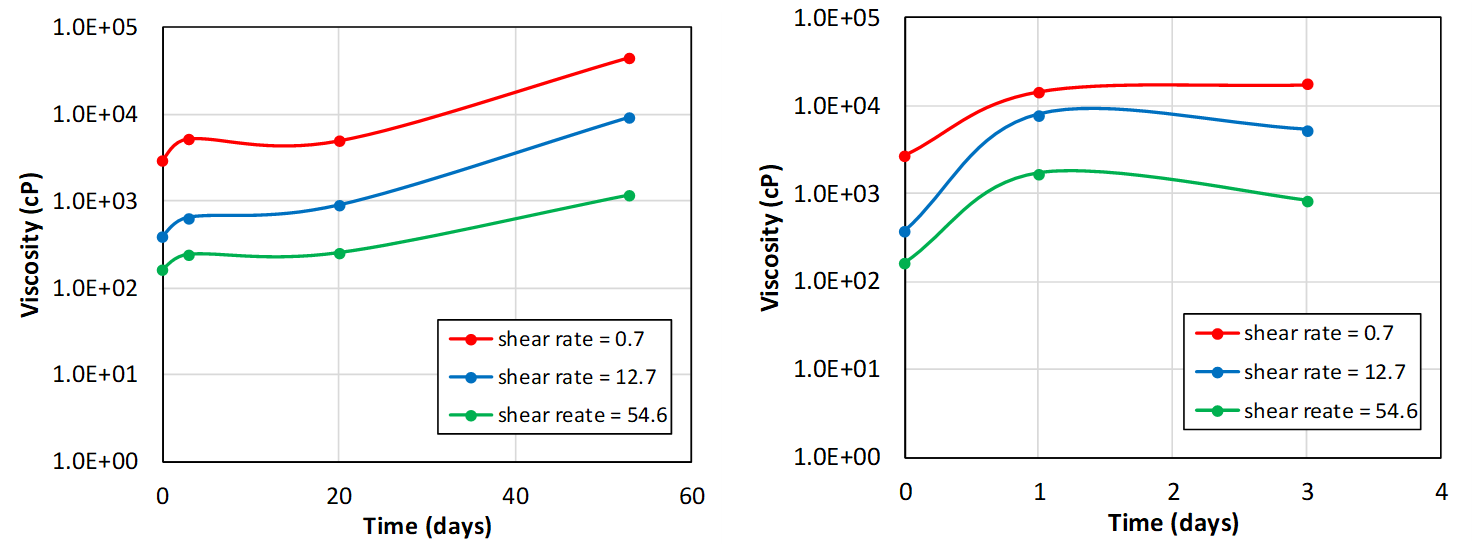
\includegraphics[width=1.2\textwidth]{img/cht/s38visc80.png}}
    \caption{Aging of samples in Series 38 made with Flopaam 5115 VHM/PEC and aged at 80~\celsius~(left), and of the same polymer with \ce{Cr^{3+}} (Series 1) and aged at 50~\celsius~(right).}
    \label{cht:s38visc80}
\end{figure}

By comparing Figures \ref{cht:s17visc80} and \ref{cht:s38visc80}, it can be seen that the viscosity in polymer/PEC systems made with Alcomer 24 UK as well as the ones made with Flopaam 5115 VHM showed an initial increase, and then plateaued before further increase. The period for constant viscosity lasted until at least 20 days, but could have been longer as there were no measurements between 20 and 53 days. The viscosity of Series 1 samples, aged at lower temperature, increased quickly as the result of gel formation.

Figure \ref{cht:s41visc80} compares polymer/PEC solutions where the concentration of Flopaam 5115 VHM was reduced to 0.50 wt.\% (Series 41). Series 41 was made with the same concentration of amide POSS (0.38 wt.\%) and of PVS (0.054 wt.\%) as Series 38. 

\begin{figure}
    \centering
    \makebox[\textwidth][c]{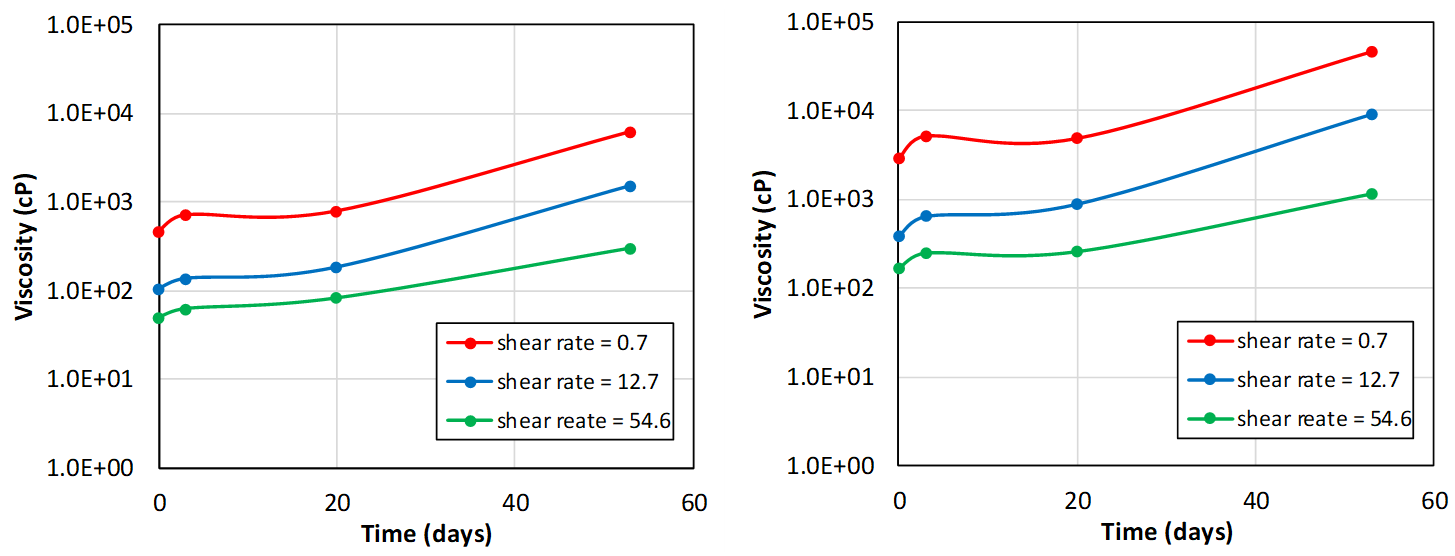
\includegraphics[width=1.2\textwidth]{img/cht/s41visc80.png}}
    \caption{Polymer/PEC solutions aged at 80~\celsius. Series 41 samples (left) and Series 38 samples (right).}
    \label{cht:s41visc80}
\end{figure}

The behavior of the Series 41 samples was comparable to that of Series 38 samples, however the measured viscosities were lower for Series 41 due to lower polymer concentration.

In Series 44, the concentrations of both amide POSS and PVS was reduced by a factor of two and the polymer concentration was kept unchanged compared to Series 17 (cf. Table \ref{tab:polyPecComp}). In Series 45, the concentrations of both amide POSS and PVS were reduced by a factor four compared to Series 17, still keeping the polymer concentration unchanged. Viscosities vs. time are compared in Figure \ref{cht:s44visc80}. The figure also shows the behaviour of the same polymer cross-linked with 104 ppm \ce{Cr^{3+}} (Series 3). Reduction of of PEC concentration reduced the rate of cross-linking. At the lowest concentration of PEC, cross-linking did not start at all in the aging period. As expected, the use of \ce{Cr^3+} as cross-linker resulted in fast gelation.

\begin{figure}
    \centering
    \makebox[\textwidth][c]{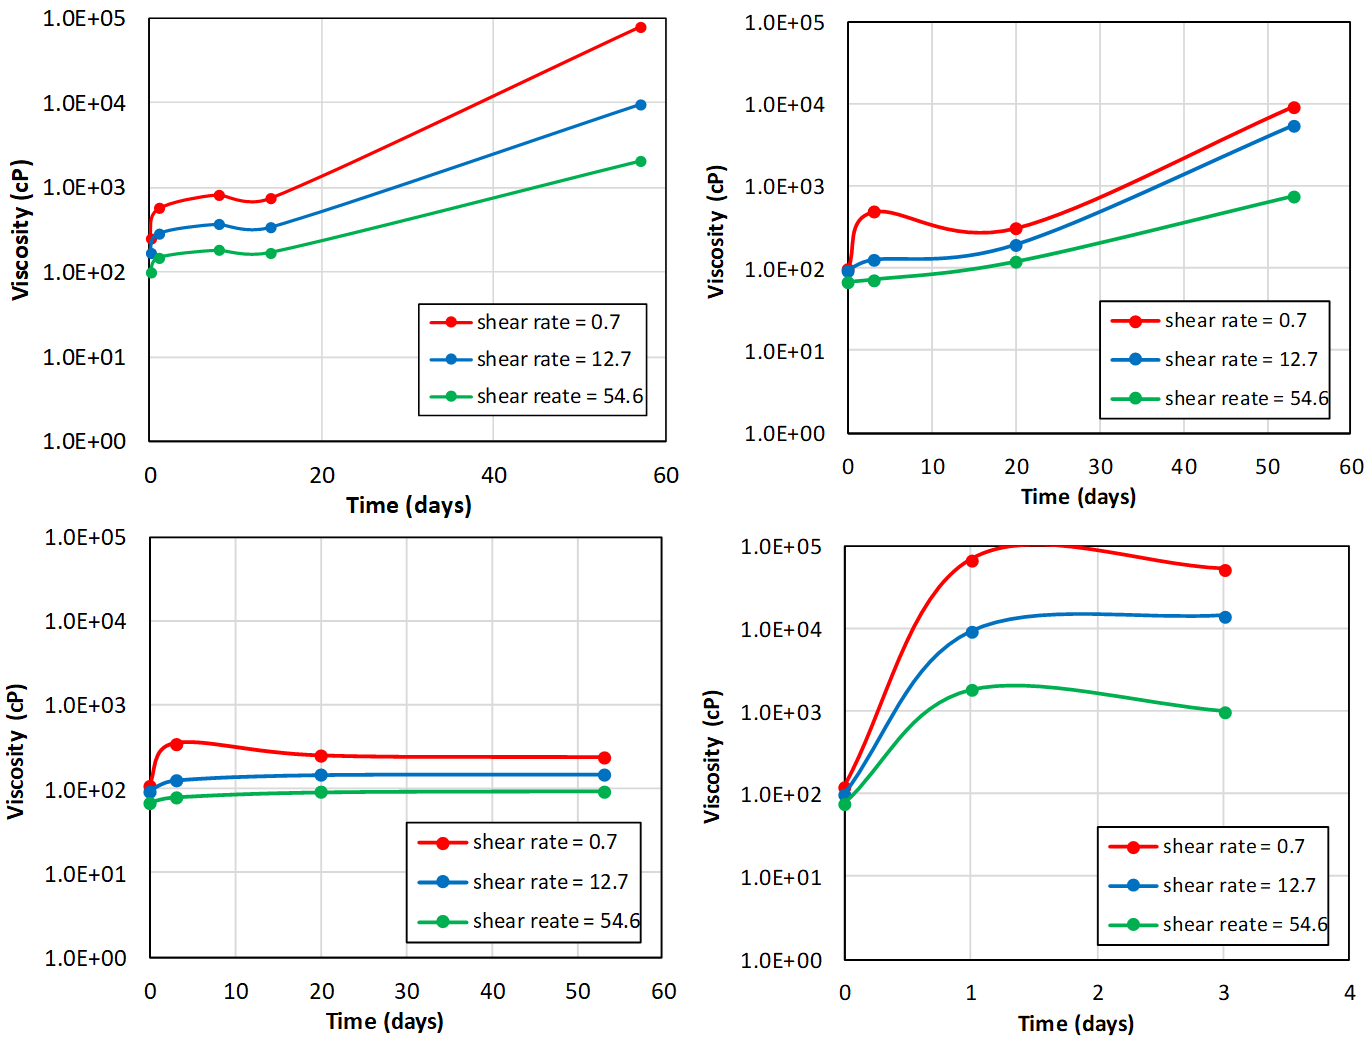
\includegraphics[width=\textwidth]{img/cht/s44visc80.png}}
    \caption{Aging of samples in Series 17 (upper left), Series 44 (upper right) and Series 45 (lower left) made with Alcomer 24 UK and aged at 80~\celsius, and of the same polymer with \ce{Cr^{3+}} (Series 3) and aged at 50~\celsius~(lower right).}
    \label{cht:s44visc80}
\end{figure}

\subsection{Gels based on lactamide POSS}
\index{lactamide POSS} Figure \ref{cht:s23visc80} shows measured viscosities for the samples collected early and at the end of the injection during Experiment 1 (cf. Section \ref{sec:inSituGelling}). Except for the sample measured after 12 days at 0.7 s$^{-1}$, a clear trend is seen in the figure showing a slow increase in viscosity the first 25 days and then a faster increase thereon.

\begin{figure} 
    \centering
    \makebox[\textwidth][c]{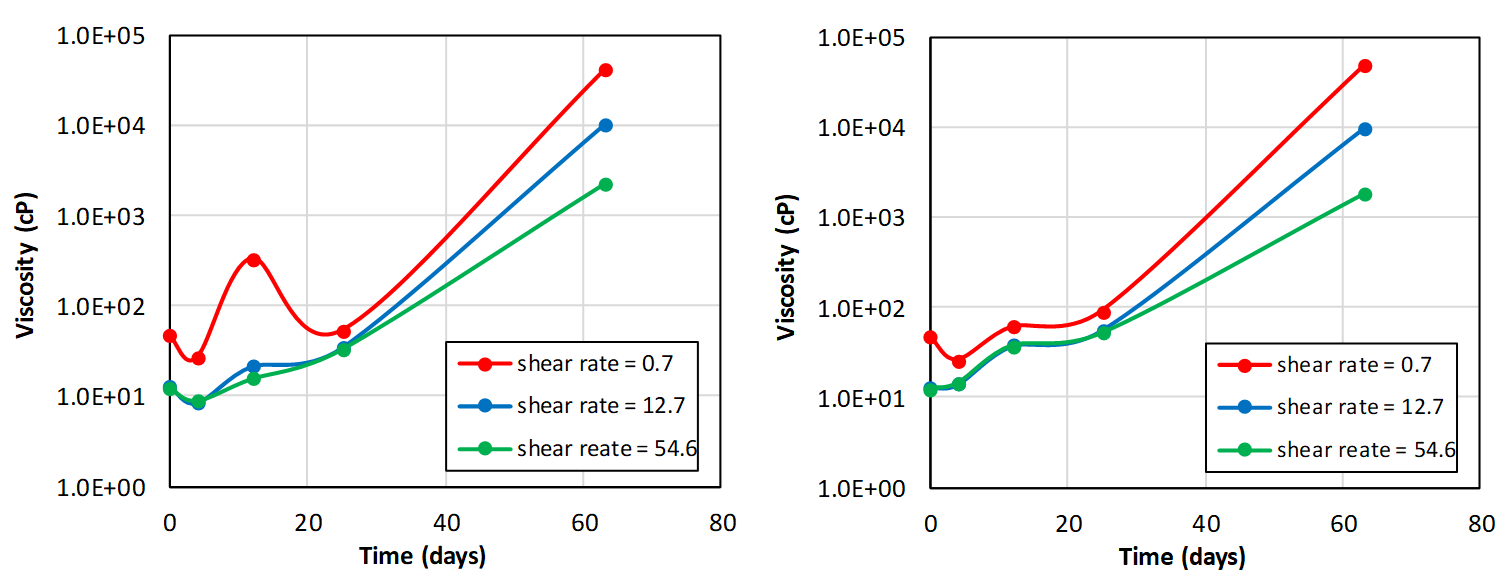
\includegraphics[width=\textwidth]{img/cht/s23visc80.png}}
    \caption{Aging of solutions in Series 23 collected during injection of nanoparticle/polymer solution in a core. Samples collected early (left) and collected at the end of the injection (right).}
    \label{cht:s23visc80}
\end{figure}

\section{Transport of polymer and nanoparticles through porous media}
\subsection{Injection of nanoparticles in Bentheimer sandstone}
\index{transport in porous media} \index{Bentheimer} Figure \ref{cht:injexp1} shows the results from injection of 1000 ppm nanoparticles in SSW as normalized concentration and normalized conductivity vs. PVs injected. The differential pressure across the core is also shown. The injection rate was 1 ml/min. The first dotted event line indicates one PV injected nanoparticle (and 100 \% SSW in the separate conductivity experiment). At 2.3 PVs injected, the nanoparticle solution is replaced with SSW (80 \% SSW for the conductivity measurement) and so forth.

\begin{figure}[h]
    \centering
    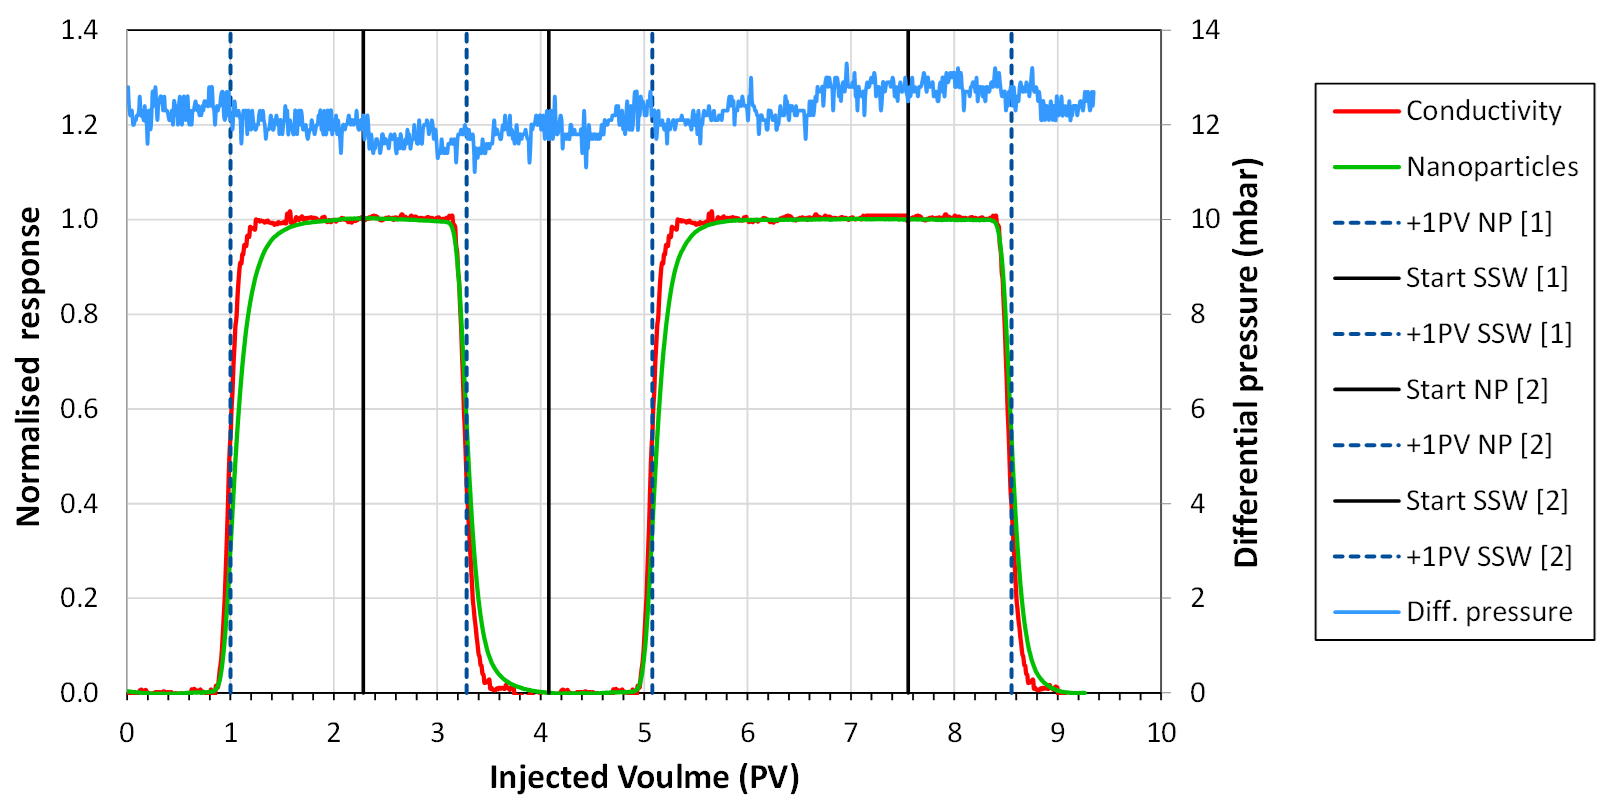
\includegraphics[width=\textwidth]{img/cht/injexp1bent.png}
    \caption{Experiment 1, injection of nanoparticles into Bentheimer sandstone}
    \label{cht:injexp1}
\end{figure}

As seen in Figure \ref{cht:injexp1}, some retention of nanoparticles occurred during the experiment. It is also seen that some of the retained matter was released during SSW flooding. In total, three flooding experiments were conducted which yielded results similar to Experiment 1 shown in Figure \ref{cht:injexp1}.

Table \ref{tab:ipvexp1} summarizes calculated IPVs and retention of nanoparticles during the experiment. The IPVs were found from the difference between the areas under the red and green curves for stages 2 and 4 of the experiment in Figure \ref{cht:injexp1} (see also Figure \ref{fig:ipvRet2}). The area under the red curves are ideally equal to one. IPVs less than zero indicate that retained nanoparticles are released during subsequent SSW flooding.

Retention of nanoparticles were found from mass balances at each stage. After Stage 1, there was an excess of 4.3 mg nanoparticles in the core, assuming that the hole pore volume was filled with nanoparticle solution. After Stage 2 some of the nanoparticles were released, leaving 2.5 mg in the core at the end of this stage. In Stage 3 more nanoparticles were injected and an excess of 5.8 mg was calculated at the end of the stage. Finally, in Stage 4 some nanoparticles are released leaving 4.7 mg in the core at the end of the experiment. By dividing the retention by the core mass, retention in mg/g rock was found.

During Stage 1, 1.89 mg nanoparticles were retained per PV nanoparticles injected, which were reduced to 2.0 mg/PV nanoparticles after SSW injection in Stage 2. During Stage 3, 0.96 mg nanoparticles were retained per PV injected at the stage. 

Finally, in the last row of Table \ref{tab:ipvexp1}, retention as percentage of injected nanoparticles at stages 1 and 3 are given as well as retention as percentage of total injected nanoparticles at the end of stages 2 and 4. 

\begin{table} % table 5.3
\small
\centering
\caption{Inaccessible pore volume (IPV) and retention of nanoparticles during Experiment 1.}
\label{tab:ipvexp1}
\begin{tabular}{c l l l l l } 
\toprule
\textbf{Quantity} & \textbf{Unit} & \textbf{Stage 1} & \textbf{Stage 2} & \textbf{Stage 3} & \textbf{Stage 4} \\ 
\midrule 
IPV         & [PV]          & -         & -0.03     & -         & -0.02     \\
Retention   & [mg]          & 4.3       & 2.5       & 5.8       & 4.7       \\ 
Retention   & [mg/g rock]   & 0.009     & 0.005     & 0.013     & 0.010     \\ 
Retention   & [mg/PV inj]   & 1.89      & -         & 0.96      & -         \\
Retention   & [\% of inj NP]& 3.6       & 2.0       & 1.8       & 1.5       \\ 
\bottomrule
\end{tabular}
\end{table}

\subsection{Injection of polymer in Bentheimer sandstone}
Figure \ref{cht:injexp2} shows the results from injection of 1000 ppm polymer as normalized concentration and normalized conductivity vs. PVs injected. The differential pressure across the core is also shown. The injection rate was 0.5 ml/min. The solid lines indicate start of a stage, and each dotted line indicates one subsequent PV. 

Figure \ref{cht:injexp2Comp1-3} compares produced normalized polymer concentration in stages 1 and 3. The conductivity response is from Stage 1. The area between the two polymer response curves represent the adsorption of polymer, cf. Figure \ref{fig:ipvRet2}.

\begin{figure}[h]
    \centering
    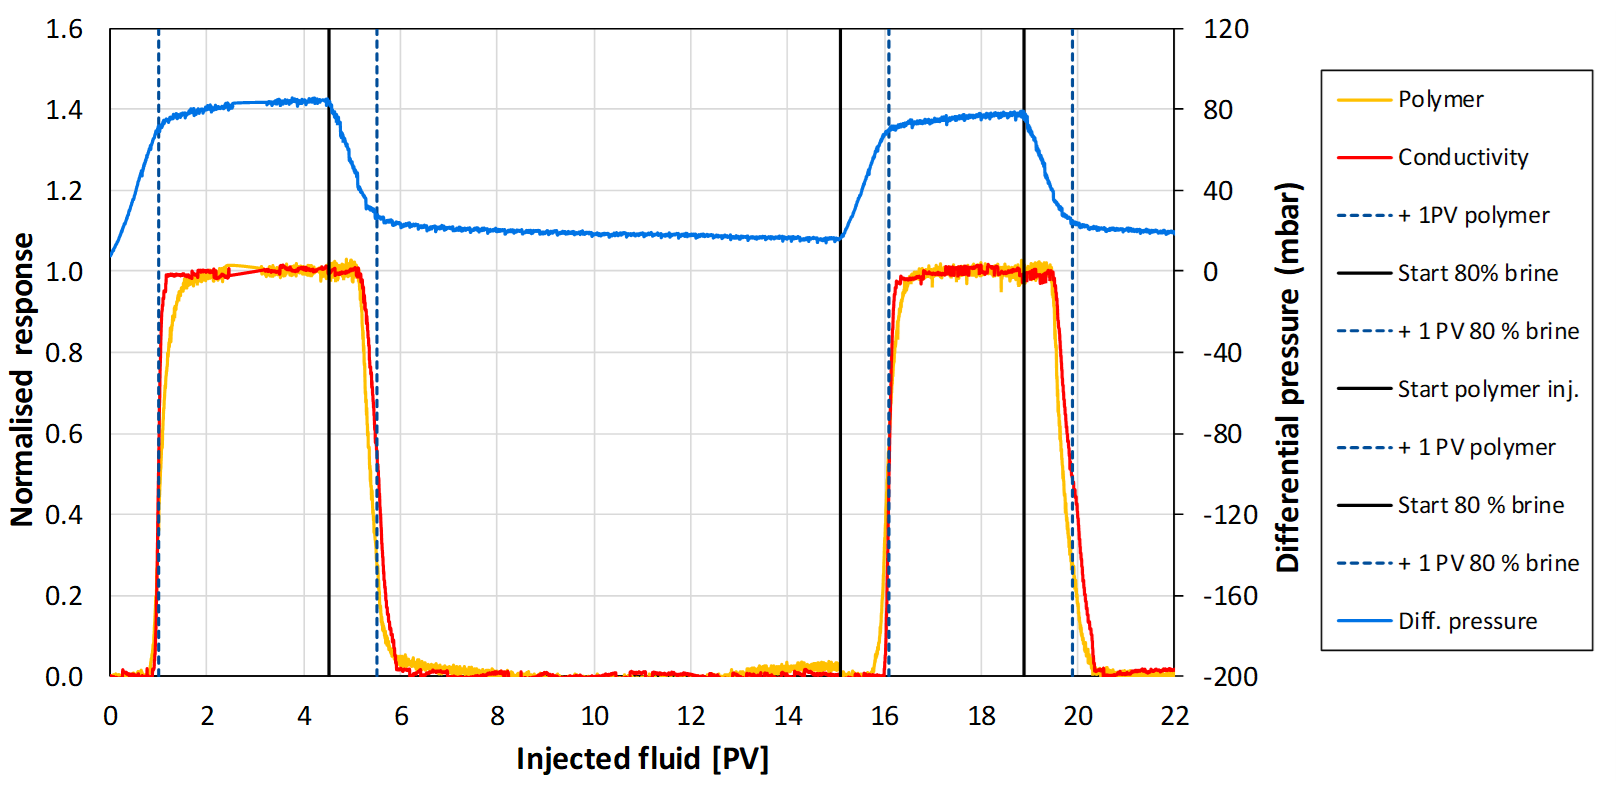
\includegraphics[width=\textwidth]{img/cht/injexp2bent.png}
    \caption{Experiment 2, injection of polymer into Bentheimer sandstone}
    \label{cht:injexp2}
\end{figure}

\begin{figure}[h!   ]
    \centering
    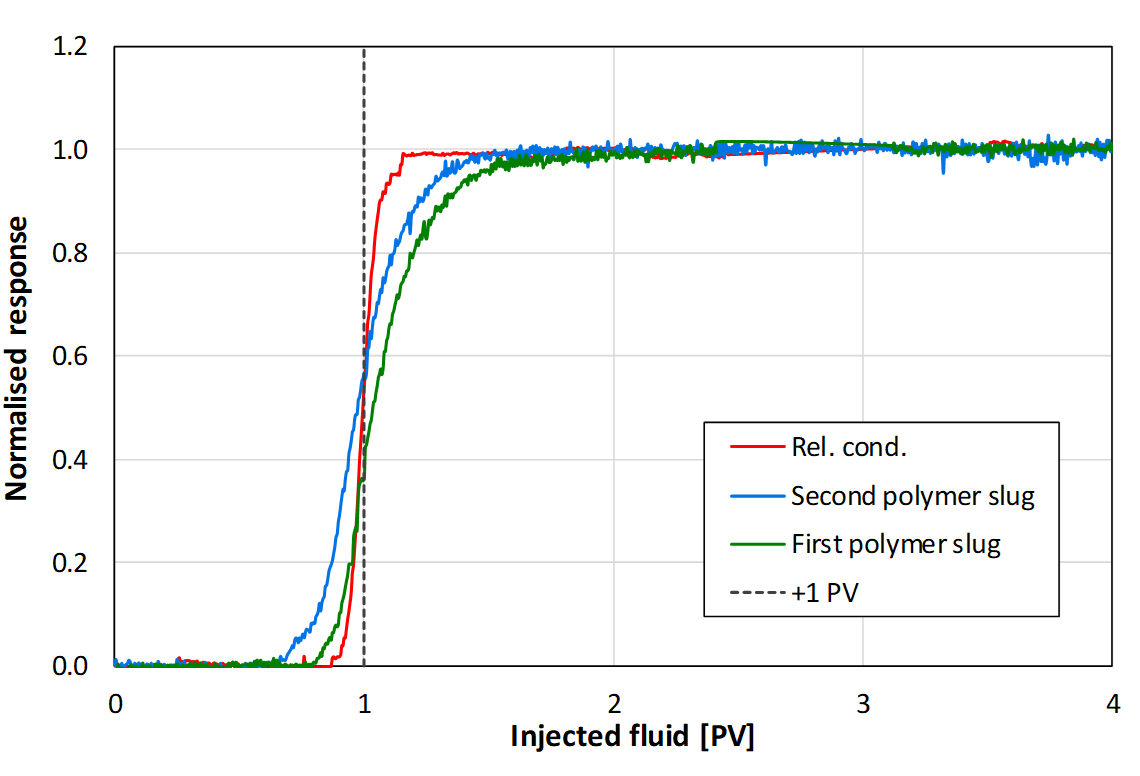
\includegraphics[width=\textwidth]{img/cht/injexp2bentComp1-3.png}
    \caption{Experiment 2, injection of polymer into Bentheimer sandstone. Comparison of polymer responses in stages 1 and 3.}
    \label{cht:injexp2Comp1-3}
\end{figure}


Table \ref{tab:ipvexp2} summarizes calculated IPVs , adsorbed polymer and mechanical entrapment of polymer during the experiment. Total retention of polymer minus adsorbed polymer is denoted mechanical entrapment. Mechanical entrapment was found from mass balances at each stage taking adsorption into account. At the end of stages 1 and 3 it was assumed that the accessible pore volume (1-IPV) was filled with polymer solution of injected concentration. Further, in the mass balances it was assumed that polymer adsorbed irreversibly to the rock. Thus, the 4.8 mg polymer adsorbed during Stage 1 remained adsorbed throughout the experiment.

\begin{table} 
\small
\centering
\caption{Inaccessible pore volume (IPV), adsorption and mechanical entrapment of polymer during Experiment 2.}
\label{tab:ipvexp2}
\begin{tabular}{c l l l l l } 
\toprule
\textbf{Quantity} & \textbf{Unit} & \textbf{Stage 1} & \textbf{Stage 2} & \textbf{Stage 3} & \textbf{Stage 4} \\ 
\midrule 
IPV                & [PV]           & -         & 0.07     & -         & -0.02     \\
Mech. entrapment   & [mg]          & 3.3       & 3.3       & 5.8       & 4.7       \\ 
Mech. entrapment   & [mg/g rock]   & 0.007     & 0.007     & 0.013     & 0.010     \\ 
Mech. entrapment   & [mg/PV inj]   & 0.74      & -         & 0.96      & -         \\
Mech. entrapment   & [\% of inj pol.]& 1.3       & 1.3       & 1.8       & 1.5       \\ 
Adsorption         & [mg]          & 4.8       &   \multicolumn{3}{c}{\multirow{2}{15em}{from difference in response curves of stages 1 and 3}}        \\
Adsorption         & [mg/g rock]   & 0.10      &  \multicolumn{3}{c}{}    \\ 
\bottomrule
\end{tabular}
\end{table}

After Stage 1 there was 3.3 mg polymer trapped in the core. This was increased to 10 mg during the Stage 3 polymer injection. During Stage 1 polymer injection 1.3 \% of the polymer that was injected was mechanically entrapped. At Stage 3, 3.3 \% of the polymer injected was trapped. The 10 mg polymer mechanically entrapped at the end of Stage 4 correspond to 2.3 \% of the in total 448 mg polymer that was injected during the experiment. In calculation of the IPVs it was assumed that no entrapped polymer was released.

\subsection{Injection of nanoparticles and polymer in Bentheimer sandstone}

Figure \ref{cht:injexp3bent} shows the results from injection of 2000 ppm nanoparticles and 500 ppm polymer as normalized concentration and normalized conductivity vs. PVs injected. The differential pressure across the core is also shown. The injection rate was 0.27 ml/min. The nanoparticle and polymer concentrations were set in order to get a practical calibration curve, cf. Figure 5.5. The UV absorption of polymer was much higher than for nanoparticles.

\begin{figure}[h]
    \centering
    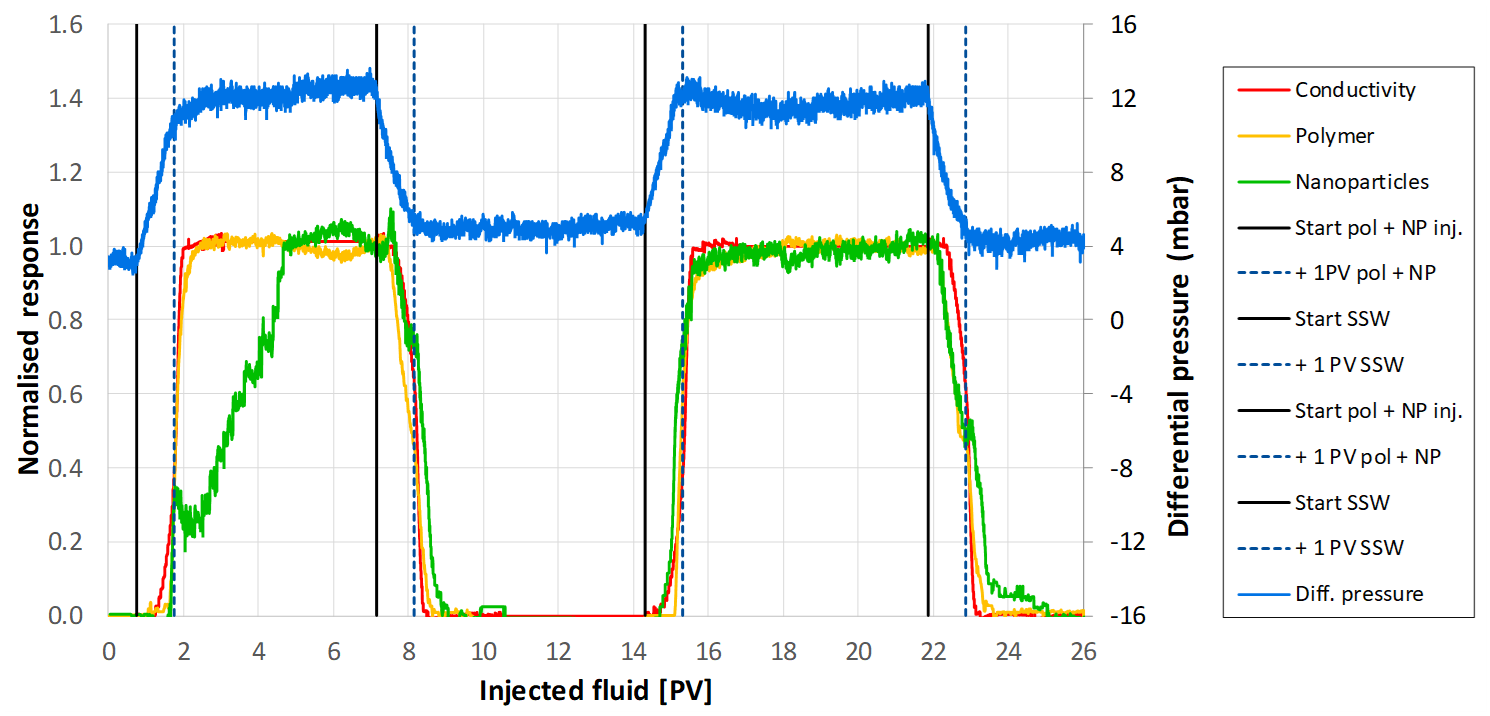
\includegraphics[width=\textwidth]{img/cht/injexp3bent.png}
    \caption{Experiment 3, injection of nanoparticles and polymer into Bentheimer sandstone.}
    \label{cht:injexp3bent}
\end{figure}

The most striking results in Figure \ref{cht:injexp3bent} is the missing part of the normalized response of nanoparticles in the first part of Stage 1. A response more like the Stage 3 response was expected based on the experiment with only nanoparticles, cf. Figure \ref{cht:injexp1}. However, the shown response is used in the mass balance calculations.
%%%

Mass balance calculations for nanoparticles and polymer are shown in Table \ref{tab:ipvexp3} and Table \ref{tab:ipvexp3pol}. Absorption of polymer was calculated from the polymer responses in Stages 1 and 3, cf.  Figure \ref{cht:injexp3bentPol}. As the responses did not coincide completely at relative responses of 1.0 adsorption was estimated in two different manners. In the first approach, the areas under both curves were found by numerical integration and subtracted from the total pore volumes polymer injected in the two stages.  This gave a difference of 0.0034 PV or 0.09 mg polymer. In the second approach, the difference in injected pore volumes at a relative response of 0.5 was used. This difference was 0.086 PV or 2.23 mg polymer. This figure was used in the mass balance calculations.

From Table  \ref{tab:ipvexp3} it is seen that there apparently was a significant retention of nanoparticles during Stage 1. Some of the retained mater was released during Stage 2 resulting in a negative IPV. The retention during stage 3 was low, only 0.87 \% of the injected matter. More nanoparticles were released in Stage 3, again giving a negative IPV. The overall retention of nanoparticles amounted to 7.9 \% of injected matter.

\begin{table} 
\small
\centering
\caption{Inaccessible pore volume (IPV) and retention of nanoparticles during Experiment 3.}
\label{tab:ipvexp3}
\begin{tabular}{c l l l l l } 
\toprule
\textbf{Quantity} & \textbf{Unit} & \textbf{Stage 1} & \textbf{Stage 2} & \textbf{Stage 3} & \textbf{Stage 4} \\ 
\midrule 
IPV         & [PV]          & -         & -0.16     & -         & -0.08     \\
Retention   & [mg]          & 153       & 125       & 132       & 114       \\ 
Retention   & [mg/g rock]   & 0.35      & 0.28     & 0.30     & 0.26     \\ 
Retention   & [mg/PV inj]   & 0.47      & -         & 0.02      & -         \\
Retention   & [\% of inj NP]& 23        & 19       & 0.87       & 7.9       \\ 
\bottomrule
\end{tabular}
\end{table}

\begin{table}[h!]
\small
\centering
\caption{Inaccessible pore volume (IPV), adsorption and mechanical entrapment of polymer during Experiment 3.}
\label{tab:ipvexp3pol}
\begin{tabular}{c l l l l l } 
\toprule
\textbf{Quantity} & \textbf{Unit} & \textbf{Stage 1} & \textbf{Stage 2} & \textbf{Stage 3} & \textbf{Stage 4} \\ 
\midrule 
IPV                & [PV]           & -         & 0.07     & -         & 0.13     \\
Mech. entrapment   & [mg]          & 2.5       & 2.5      & 6.88       & 6.88       \\ 
Mech. entrapment   & [mg/g rock]   & 0.0057   & 0.0057     & 0.016     & 0.016     \\ 
Mech. entrapment   & [mg/PV inj]   & 0.39      & -         & 0.58      & -         \\
Mech. entrapment   & [\% of inj pol.]& 1.5       & 1.5       & 2.24       & 1.90       \\ 
Adsorption         & [mg]          & 2.22      &   \multicolumn{3}{c}{\multirow{2}{15em}{from difference in response curves of stages 1 and 3}}        \\
Adsorption         & [mg/g rock]   & 0.005      &  \multicolumn{3}{c}{}    \\ 
\bottomrule
\end{tabular}
\end{table}

\begin{figure}[h!]
    \centering
    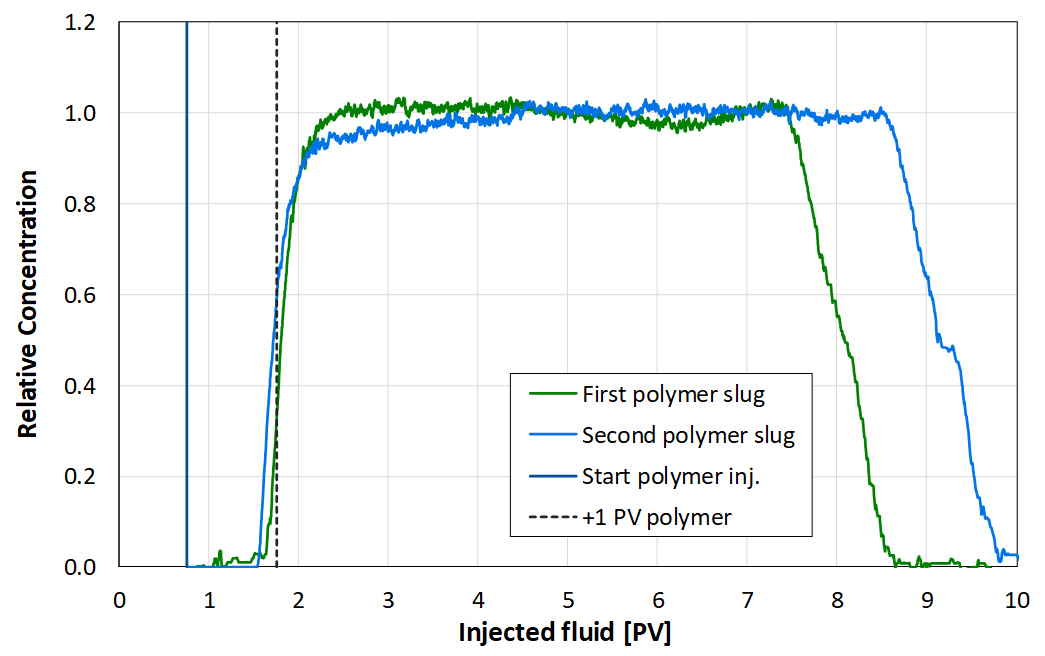
\includegraphics[width=.85\textwidth]{img/cht/injexp3bentPol.png}
    \caption{Experiment 3 injection of polymer into Bentheimer sandstone. Comparison of polymer responses in stages 1 and 3.}
    \label{cht:injexp3bentPol}
\end{figure}

The adsorption, IPVs and mechanically entrapped polymer in Experiment 3 are all of the same magnitude as for Experiment 2 (only polymer injection). The differences are likely within the uncertainty of the measurements and following calculations that are based on the numerical integration of response curves.



\subsection{Injection of nanoparticles in Berea sandstone}
In the experiments with nanoparticle injection into \index{Berea} Berea sandstone severe problems with both the refractive index and UV detectors were experienced. In total three experiments were conducted. The problem was that the detector responses did not reach the bypass values measured after stages 1 and 3. Furthermore, the bypass values were not identical after the two stages. For example; during Stage 1 the maximum refractive index response measured was 60.4, whereas the bypass value was 64.1. for Stage 3 the corresponding measurements were 78.2 and 82.0. Thus, two approaches were used to calculated IPV and retention. In the first approach, the detector response was normalized to the bypass values, whereas in the second approach, the maximum measured values during flooding through the core were used. The response curves for the two approaches are shown in Figure \ref{cht:injexp4ber1} and Figure \ref{cht:injexp4ber2}. 

\begin{figure}[h]
    \centering
    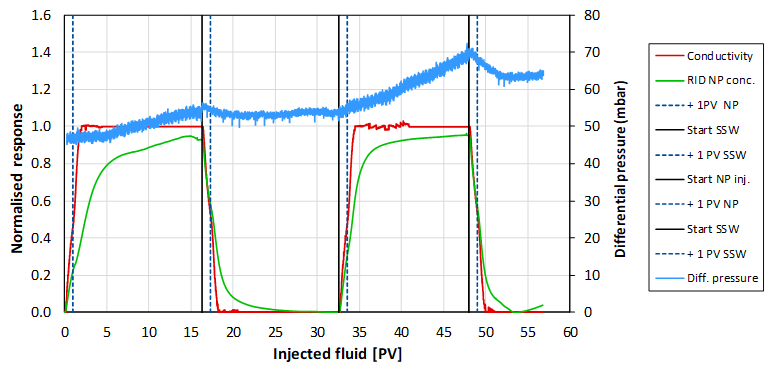
\includegraphics[width=\textwidth]{img/cht/injexp4ber1.png}
    \caption{Experiment 4, injection of nanoparticles into Berea sandstone. Detector response normalized to bypass values.}
    \label{cht:injexp4ber1}
\end{figure}

\begin{figure}[h]
    \centering
    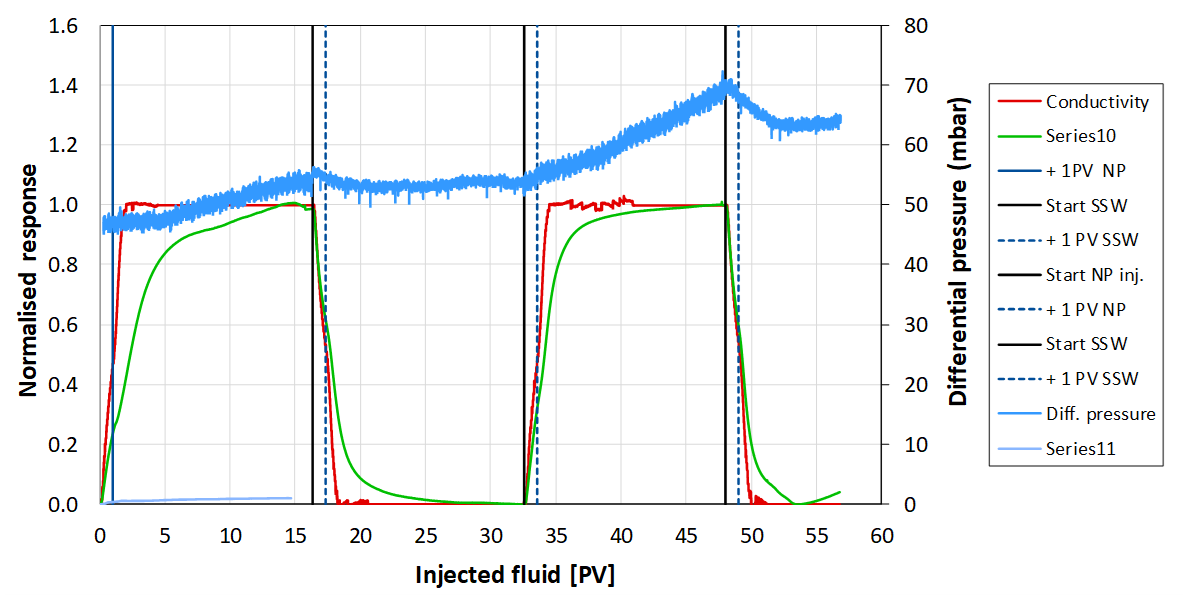
\includegraphics[width=\textwidth]{img/cht/injexp4ber2.png}
    \caption{Experiment 4, injection of nanoparticles into Berea sandstone. Detector response normalized to maximum measured values during nanoparticle injection.}
    \label{cht:injexp4ber2}
\end{figure}

Figure \ref{cht:IPVber} shows IPVs calculated for different experiments and calculation approaches. The average value and its standard deviation is also shown. With one exception, the IPVs are negative, indicating release of retained nanoparticles during SSW injection at stages 2 and 4. Retention of nanoparticles after the various stages are shown in Figure \ref{cht:retentionBer}. The values for Stage 3 is retention at this stage, whereas the Stage 4 retention is the amount of nanoparticles at the end of the stage in percentage of the total amount injected at stages 1 and 3.

\begin{figure}[h!]
    \centering
    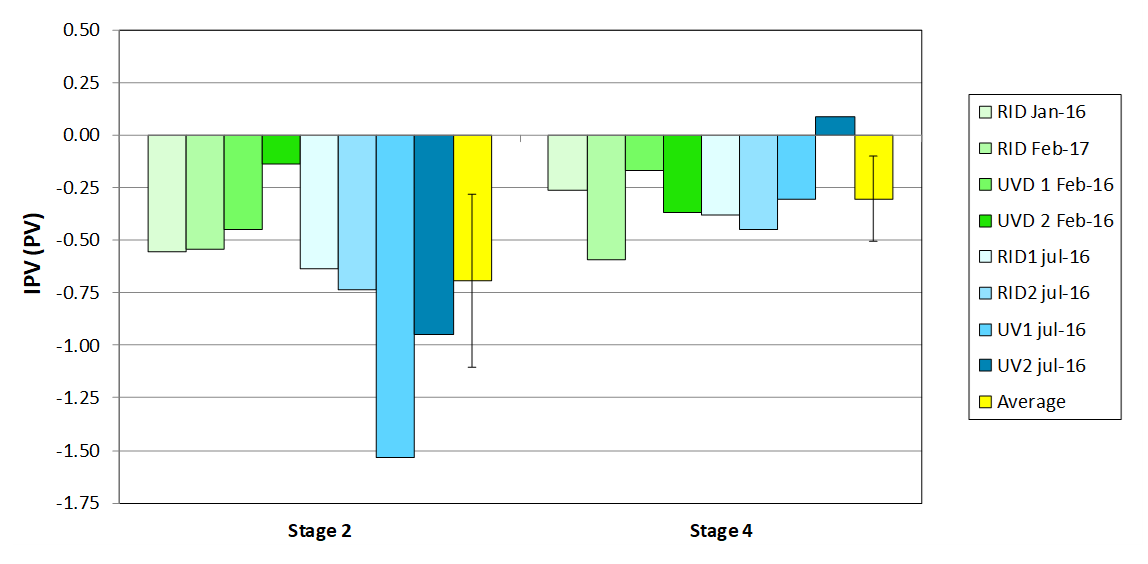
\includegraphics[width=\textwidth]{img/cht/IPVber.png}
    \caption{IPVs calculated for injection of nanoparticles into Berea sandstone. Results from different experiments and calculation methods.}
    \label{cht:IPVber}
\end{figure}

\begin{figure}[h!]
    \centering
    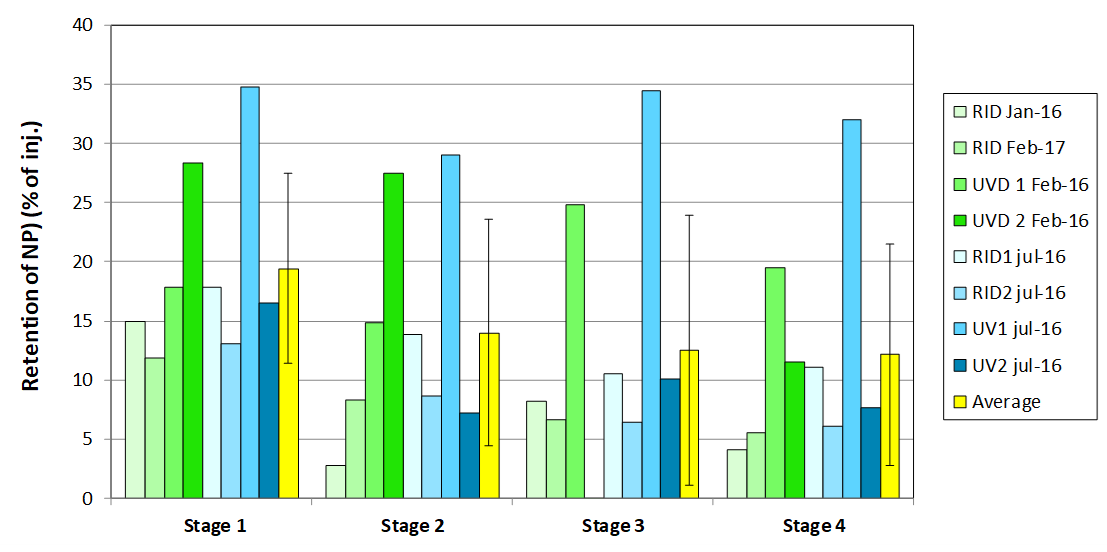
\includegraphics[width=\textwidth]{img/cht/retentionBer.png}
    \caption{Retention of nanoparticles during injection into Berea sandstone. Results from different experiments and calculation methods.}
    \label{cht:retentionBer} % 5.14
\end{figure}

From Figures \ref{cht:IPVber} and \ref{cht:retentionBer} it is seen that the two UV measurements gave significantly higher retention compared to the others. The true values can thus be lower than the averages.

The very fast conductivity responses and significantly tailing, as seen in Figure 5.11 and Figure 5.12, indicate that the rock material was fairly in-homogeneous. During injection of SSW (with the core initially at 80 \% SSW) the conductivity started to increase already after 0.16 PV injection as shown in Figure \ref{cht:CondBerNorm}. Conductivity was measured before nanoparticle injection.

\begin{figure}[p]
    \centering
    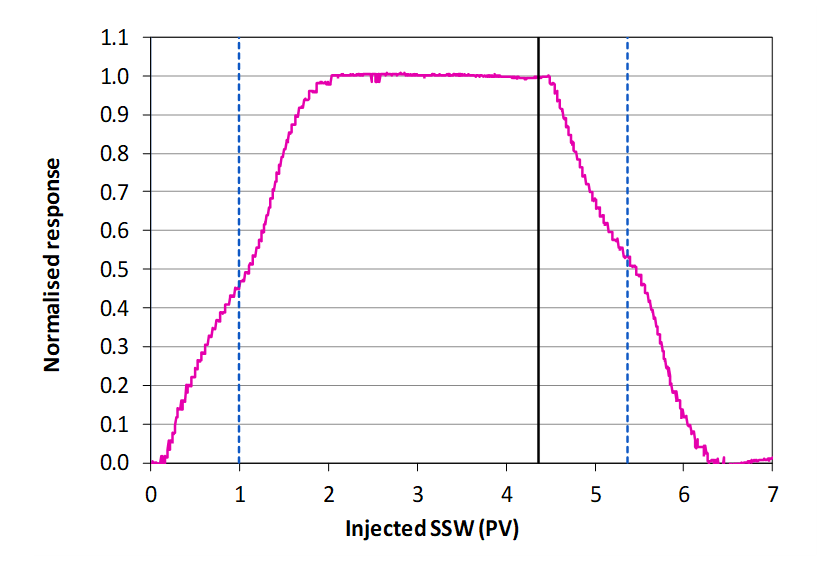
\includegraphics[width=\textwidth]{img/cht/CondBerNorm.png}
    \caption{Normalized conductivity response for Berea sandstone core (July-16).}
    \label{cht:CondBerNorm}
\end{figure}

\subsection{Injection of polymer in Berea sandstone}
Figure \ref{cht:injexp5ber1} shows the results from injection of 1000 ppm polymer as normalized concentration and normalized conductivity vs. PVs injected. The differential pressure across the core is also shown. The injection rate was 0.27 ml/min.

\begin{figure}[p]
    \centering
    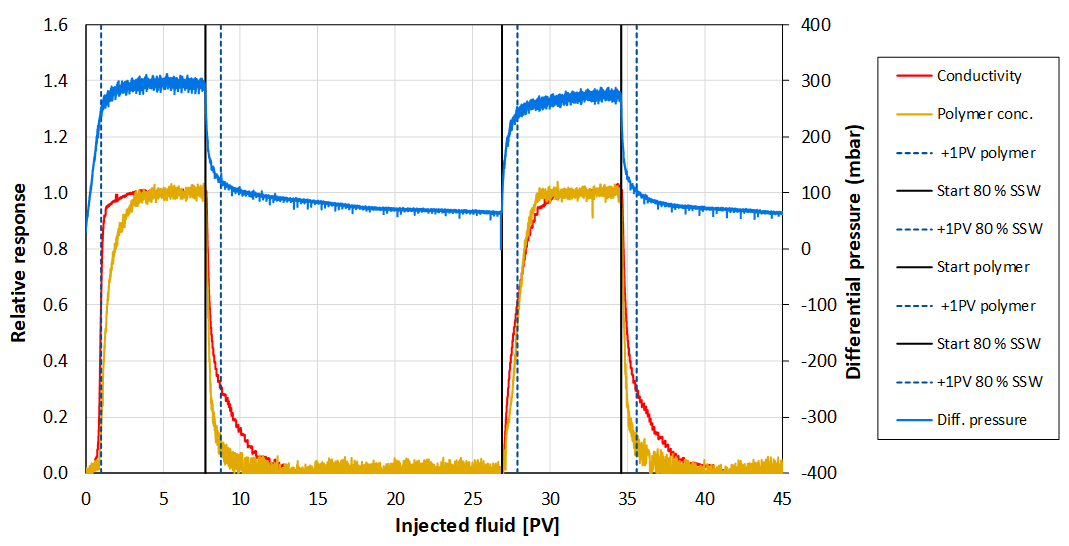
\includegraphics[width=\textwidth]{img/cht/injexp5ber1.png}
    \caption{Experiment 5, injection of polymer into Berea sandstone.}
    \label{cht:injexp5ber1}
\end{figure}

Figure \ref{cht:injexp5ber2} compares produced normalized polymer concentration in stages 1 and 3. The conductivity response is from Stage 1. The area between the two polymer response curves represent the adsorption of polymer. Note the fast response to polymer in the second slug (Stage 3).
 
\begin{figure}[h!]
    \centering
    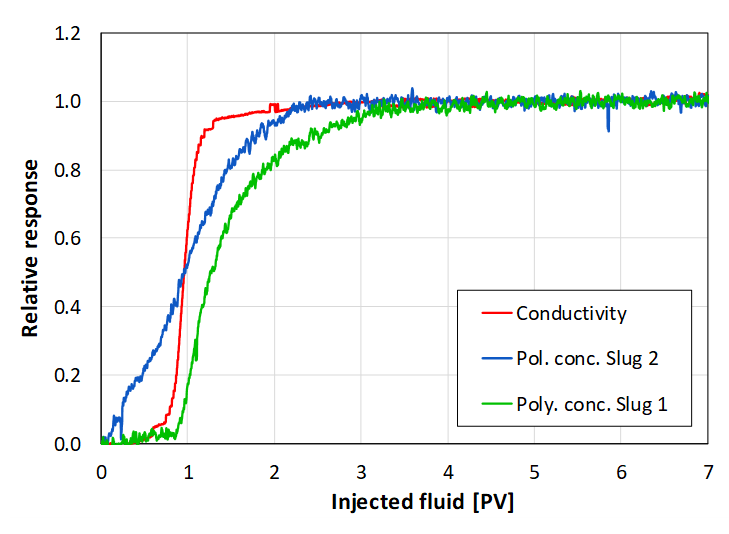
\includegraphics[width=\textwidth]{img/cht/injexp5ber2.png}
    \caption{Experiment 5 injection of polymer into Berea sandstone. Comparison of polymer responses in stages 1 and 3.}
    \label{cht:injexp5ber2}
\end{figure}

Table \ref{tab:ipvexp5pol} summarizes calculated IPVs, adsorbed polymer and mechanical entrapment of polymer during the experiment. Total retention of polymer minus adsorbed polymer is denoted mechanical entrapment. Mechanical entrapment was found from mass balances at each stage taking adsorption into account. At the end of stages 1 and 3 it was assumed that the accessible pore volume (1-IPV) was filled with polymer solution of injected concentration. Further, in the mass balances it was assumed that polymer adsorbed irreversibly to the rock. Thus, the 19.3 mg polymer adsorbed during Stage 1 remained adsorbed throughout the experiment.

After Stage 1, there remained 27.8 mg polymer trapped in the core. This was increased to 55.8 mg during the Stage 3 polymer injection. During Stage 1 polymer injection 8.3\% of the injected polymer was mechanically entrapped. At Stage 3, 12.5 \% of the injected polymer was trapped. The 55.6 mg mechanically entrapped polymer at the end of Stage 4 corresponds to 10.0\% of a total of 558 mg polymer that was injected during the experiment. In calculation of the IPVs, it was assumed that no entrapped polymer was released during SSW injection.

\begin{table}
\small
\centering
\caption{Inaccessible pore volume (IPV), adsorption and mechanical entrapment of polymer during Experiment 5.}
\label{tab:ipvexp5pol}
\begin{tabular}{c l l l l l } 
\toprule
\textbf{Quantity} & \textbf{Unit} & \textbf{Stage 1} & \textbf{Stage 2} & \textbf{Stage 3} & \textbf{Stage 4} \\ 
\midrule 
IPV                & [PV]           & -         & 0.60     & -         & 0.59     \\
Mech. entrapment   & [mg]          & 27.8       & 28.0      & 55.8       & 55.6       \\ 
Mech. entrapment   & [mg/g rock]   & 0.095   & 0.096     & 0.152     & 0.151     \\ 
Mech. entrapment   & [mg/PV inj]   & 3.59      & -         & 5.4      & -         \\
Mech. entrapment   & [\% of inj pol.]& 8.3       & 8.3      & 12.5       &10.0        \\ 
Adsorption         & [mg]          & 19.3      &   \multicolumn{3}{c}{\multirow{2}{15em}{from difference in response curves of stages 1 and 3}}        \\
Adsorption         & [mg/g rock]   & 0.04      &  \multicolumn{3}{c}{}    \\ 
\bottomrule
\end{tabular}
\end{table}

\subsection{Injection of nanoparticles and polymer in Berea sandstone}
Likewise, for the experiment with injection of nanoparticles and polymer into Berea sandstone, there was difficulties in measurement of produced nanoparticles. As for Bentheimer, the polymer concentration was determined using the response of the capillary viscometer and a calibration curve. For nanoparticles, models for refractive index and UV responses were used, similar to the model shown in Figure \ref{cht:uv}. 2000 ppm nanoparticles and 500 ppm polymer were injected with a rate of 0.50 ml/min. 

Response curves for the experiments are shown in Figure \ref{cht:injexp6ber1}, which also show measured differential pressures. For the refractive index detector, the produced nanoparticle concentration approached the injected concentration during Stage 3 and the average measured concentration in the last part of the stage was used a reference for the normalization. For the UV response, there was apparently an overshooting in produced concentration between 14 and 16 PVs and an undershooting from approximately 16 PVs and until the start of Stage 4. A reference value that cancelled the over-and undershooting was used. 

Figure \ref{cht:injexp6ber2} compares produced normalized polymer concentration in stages 1 and 3. The area between the two polymer response curves represent the adsorption of polymer. Note the fast response to polymer in the second slug (Stage 3). An almost similar fast response was also observed with only polymer in Berea sandstone (see Figure \ref{cht:injexp5ber2}).

\begin{figure}[p]
    \centering
    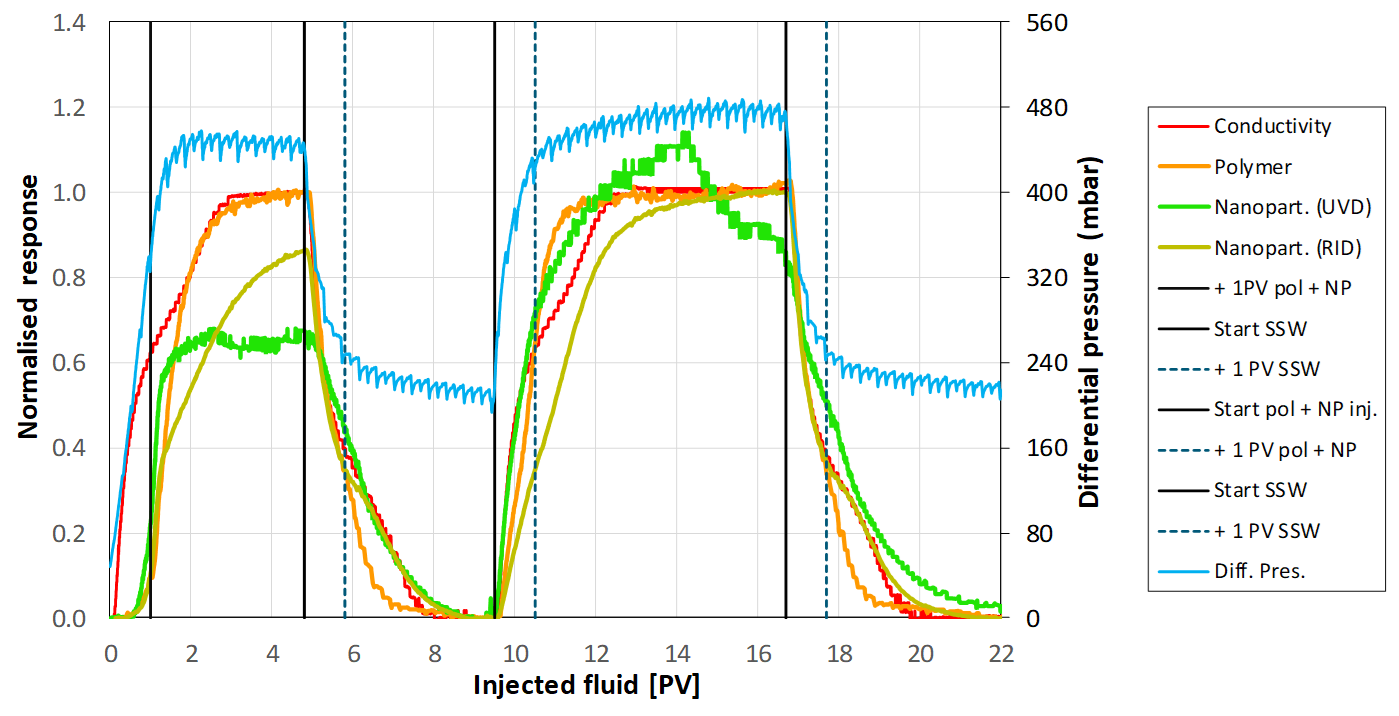
\includegraphics[width=\textwidth]{img/cht/injexp6ber1.png}
    \caption{Experiment 6, injection of nanoparticles and polymer into Berea sandstone.}
    \label{cht:injexp6ber1}
\end{figure}

\begin{figure}[p]
    \centering
    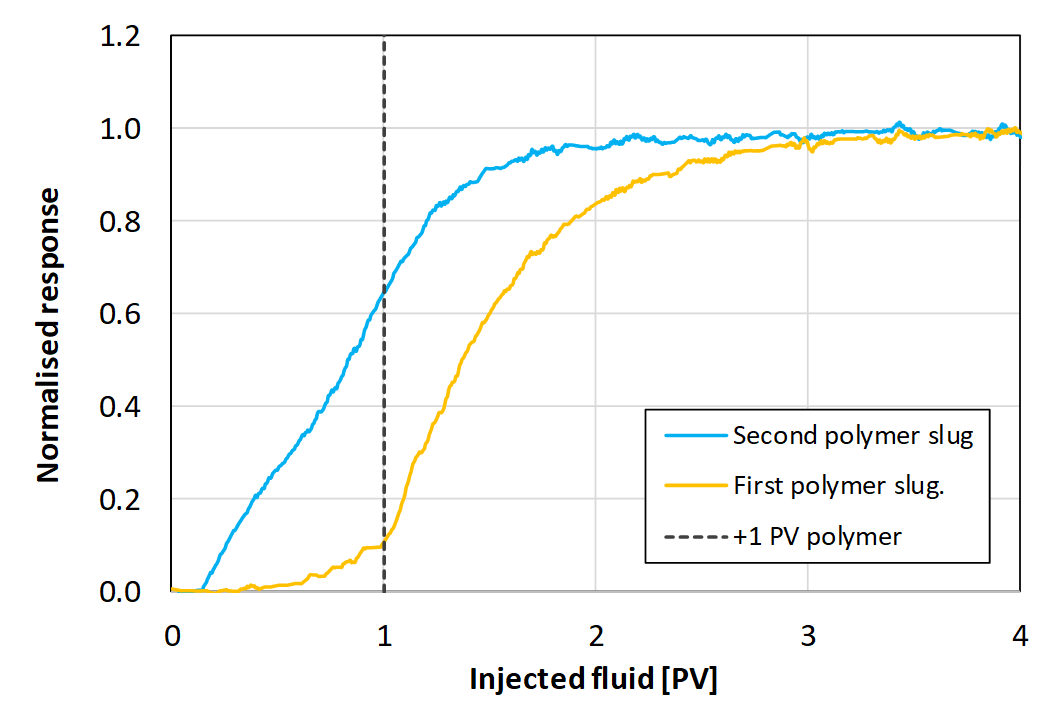
\includegraphics[width=\textwidth]{img/cht/injexp6ber2.png}
    \caption{Experiment 6, injection of nanoparticles and polymer into Berea sandstone. Comparison of polymer responses in stages 1 and 3.}
    \label{cht:injexp6ber2}
\end{figure}

Mass balance calculations for nanoparticles and polymer are shown in Table \ref{tab:ipvexp6} to Table \ref{tab:ipvexp6pol}. Absorption of polymer was calculated from the polymer responses in Stages 1 and 3, cf. Figure \ref{cht:injexp6ber2}. 

\begin{table}[p]
\small
\centering
\caption{Inaccessible pore volume (IPV) and retention of nanoparticles during Experiment 6. Calculations based on refractive index detector response.}
\label{tab:ipvexp6}
\begin{tabular}{c l l l l l } 
\toprule
\textbf{Quantity} & \textbf{Unit} & \textbf{Stage 1} & \textbf{Stage 2} & \textbf{Stage 3} & \textbf{Stage 4} \\ 
\midrule 
IPV         & [PV]          & -         & 0.04     & -         & -0.04     \\
Retention   & [mg]          & 128.98    & 132.66   & 216.97       & 214.01       \\ 
Retention   & [mg/g rock]   & 0.268     & 0.276    & 0.451     & 0.445     \\ 
Retention   & [mg/PV inj]   & 26.88     & -        & 11.72      & -         \\
Retention   & [\% of inj NP]& 30.1      & 31.0     & 0.8713.1       & 20.0       \\ 
\bottomrule
\end{tabular}
\end{table}


\begin{table}[p]
\small
\centering
\caption{Inaccessible pore volume (IPV) and retention of nanoparticles during Experiment 6. Calculations based on UV detector response.}
\label{tab:ipvexp6uv}
\begin{tabular}{c l l l l l } 
\toprule
\textbf{Quantity} & \textbf{Unit} & \textbf{Stage 1} & \textbf{Stage 2} & \textbf{Stage 3} & \textbf{Stage 4} \\ 
\midrule 
IPV         & [PV]          & -         & -0.01     & -         & -0.34     \\
Retention   & [mg]          & 152.6     & 122.9     & 102.0     & 71.7       \\ 
Retention   & [mg/g rock]   & 0.32      & 0.26      & 0.21      & 0.15     \\ 
Retention   & [mg/PV inj]   & 31.8      & -         & -2.9      & -         \\
Retention   & [\% of inj NP]& 35.6      & 28.7      & -3.2      & 6.7       \\ 
\bottomrule
\end{tabular}
\end{table}

\begin{table}[p]
\small
\centering
\caption{Inaccessible pore volume (IPV), adsorption and mechanical entrapment of polymer during Experiment 6.}
\label{tab:ipvexp6pol}
\begin{tabular}{c l l l l l } 
\toprule
\textbf{Quantity} & \textbf{Unit} & \textbf{Stage 1} & \textbf{Stage 2} & \textbf{Stage 3} & \textbf{Stage 4} \\ 
\midrule 
IPV                & [PV]           & -         & 0.23     & -         & 0.19     \\
Mech. entrapment   & [mg]          & 1.1       & 1.1      & 1.3       & 1.3       \\ 
Mech. entrapment   & [mg/g rock]   & 0.0024   & 0.0024     & 0.0028     & 0.0028     \\ 
Mech. entrapment   & [mg/PV inj]   & 0.24      & -         & 0.02      & -         \\
Mech. entrapment   & [\% of inj pol]& 1.07       & 1.7       & 0.11       & 1.50       \\ 
Adsorption         & [mg]          & 15.6      &   \multicolumn{3}{c}{\multirow{2}{15em}{from difference in response curves of stages 1 and 3}}        \\
Adsorption         & [mg/g rock]   & 0.03      &  \multicolumn{3}{c}{}    \\ 
\bottomrule
\end{tabular}
\end{table}


From Figure \ref{cht:injexp6ber1},  Table \ref{tab:ipvexp6uv} and Table \ref{tab:ipvexp6pol} it is seen that there apparently was a significant retention of nanoparticles, especially during Stage 1. Some of the retained mater was released during Stage 4 resulting in a negative IPV. The IPVs calculated from Stage 2 are close to zero. The overall retention of nanoparticles amounted, on average, to 13.3 ± 6.7 \% of injected matter.

The adsorption of polymer was of the same magnitude compared to Experiment 5 with only polymer injection (Table \ref{tab:ipvexp5pol}). However, The IPVs and mechanically entrapped polymer were significant lower.

 \subsection{Summary of core flooding experiments}
The absolute permeabilities of the cores used in the flooding experiments were determined before and after the experiments with nanoparticle and/or polymer injection. The residual resistance factor is defined by the ratio of initial and final permeability for the experiment. The results are shown in Figure \what [5.1]. In total three experiments were conducted with nanoparticles and Berea sandstone but only two determinations of residual resistance factors were done (Berea NP1 and Berea NP2).

As seen in Figure \ref{cht:rrf} contact with only nanoparticles did not change the permeability significantly. Contact with polymer reduced the permeability, especially for the Bentheimer core. The effect of adding nanoparticles to the polymer had different effects on the two different core materials. The decrease in the residual resistance factor for Bentheimer questions the value obtained with only polymer.

Figure \ref{cht:polAds} shows the results from the determination of polymer adsorption. As expected, the adsorption was much less for the almost clean high permeability Bentheimer sandstone compared to Berea sandstones that had lower permeability and most likely significantly higher specific surface area (m2/g rock) It is known that Berea also contain significant amounts of clay minerals.

\begin{figure}[p]
    \centering
    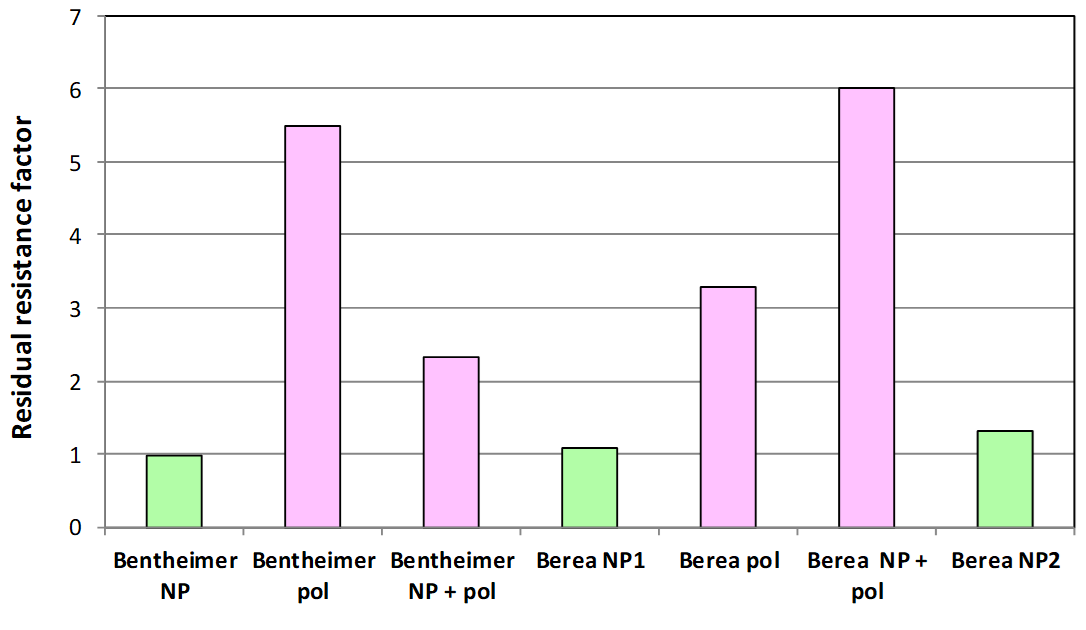
\includegraphics[width=\textwidth]{img/cht/rrf.png}
    \caption{Residual resistance factors.}
    \label{cht:rrf}
\end{figure}

\begin{figure}[p]
    \centering
    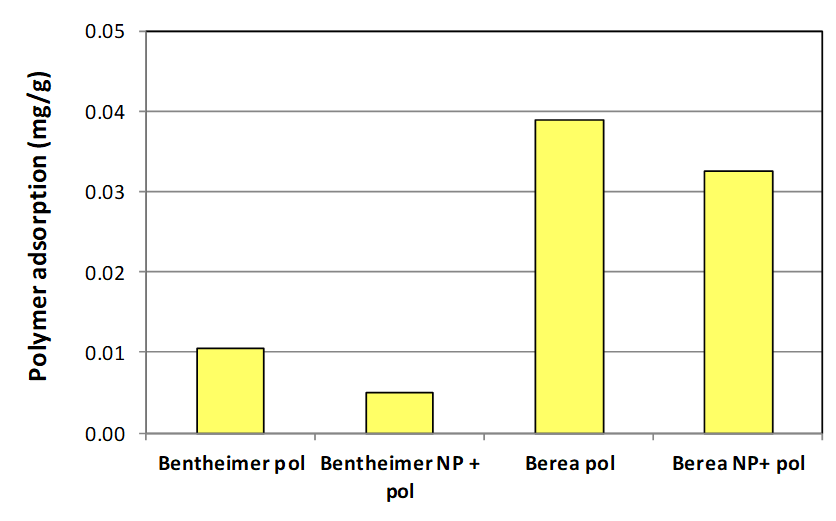
\includegraphics[width=\textwidth]{img/cht/polAds.png}
    \caption{Residual resistance factors.}
    \label{cht:polAds}
\end{figure}

The inaccessible pore volumes determined are shown in Figure \ref{cht:ipvPol}. For Bentheimer sandstone the IPVs were low and close to the same with and without nanoparticles in the injected fluid. For Berea, the IPV decreased when nanoparticles were added. 

The IPV is a measure for the fraction of the pores that were too small for the large polymer molecules to enter. It is difficult to understand how nanoparticles affected the polymer to enter smaller pores unless the polymer molecules curled up and got lower effective particle diameters in their presence. However, the differential pressure towards the end of stages 1 and 3 were higher with nanoparticles, but not more than the different rates used in the two experiments should give (cf. Figure \ref{cht:injexp5ber1} and Figure \ref{cht:injexp6ber1}). 

\begin{figure}[p]
    \centering
    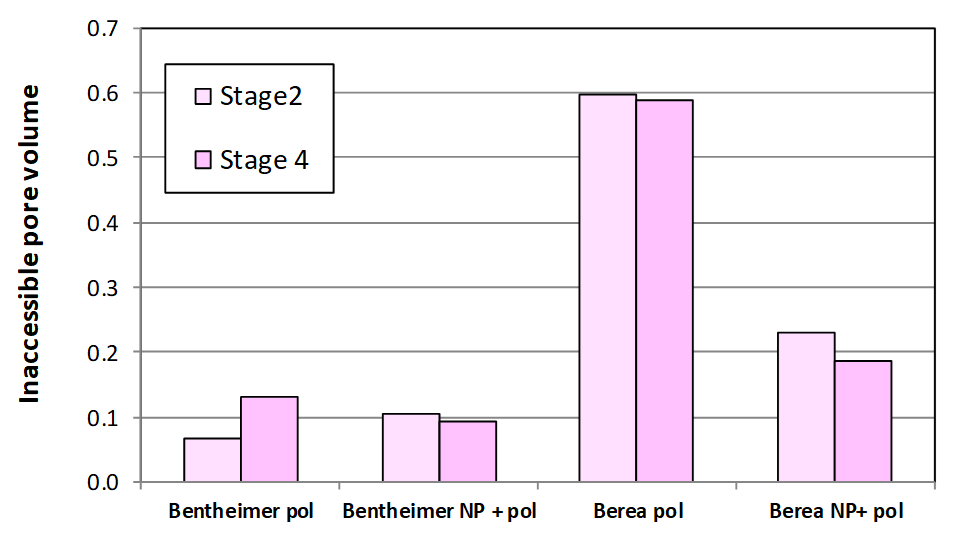
\includegraphics[width=\textwidth]{img/cht/ipvPol.png}
    \caption{Residual resistance factors.}
    \label{cht:ipvPol}
\end{figure}

IPVs were also calculated for nanoparticles. Also in this case IPVs were calculated based on the integral under the production curves as shown in Figure \what [5.2]. In all mass balance equations, it was assumed that the nanoparticles entered the whole pore volume. and the IPVs thus has a different physical meaning than for polymer. As seen in Figure \ref{cht:ipvNP} most of the IPVs are negative. A negative IPV means that more than one pore volume of nanoparticles was produced during SSW flooding, i.e. some of the nanoparticles retained during injection was released during the subsequent SSW flooding.

For some experiments, the IPV s were calculated based on both refractive index and UV detector responses, and different interpretations of the detector response. The values shown in Figure \ref{cht:ipvNP} are average values and the standard deviations are indicated by arrow bars. The results for Berea NP1 are averages for the experiments conducted in January and February 2016, whereas Berea NP2 are average results for the experiment carried out in June 2016.

\begin{figure}[p]
    \centering
    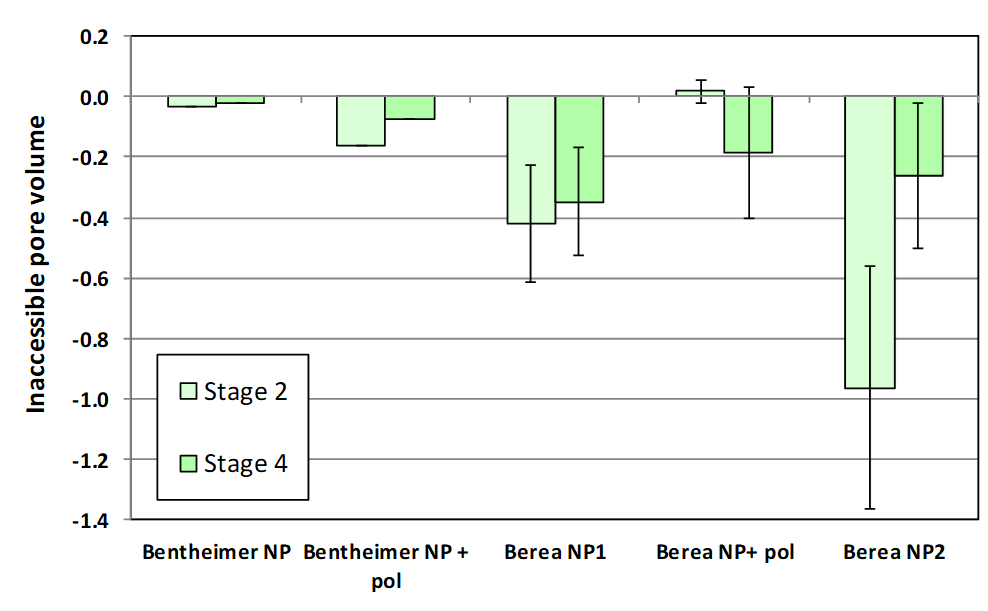
\includegraphics[width=\textwidth]{img/cht/ipvNP.png}
    \caption{Residual resistance factors.}
    \label{cht:ipvNP} % 5.23
\end{figure}

As seen in Figure \ref{cht:ipvNP}, the IPV values for nanoparticles were negative, but low for Bentheimer sandstone. For Berea sandstone, the IPVs were much lower and the uncertainty in the results are significant. 

Figure \ref{cht:retentionMech} shows the retention of nanoparticles and mechanical entrapment of polymer during all experiments. For nanoparticles in Berea sandstone the average values shown in Figure \ref{cht:retentionBer} are used. For other experiments where more than one datasets exist average values are also used. The two groups of bars to the left in the figure are for experiments where only nanoparticles or only polymer was injected. The two groups to the right are for injection of mixtures of nanoparticles and polymer.

\begin{figure}[h]
    \centering
    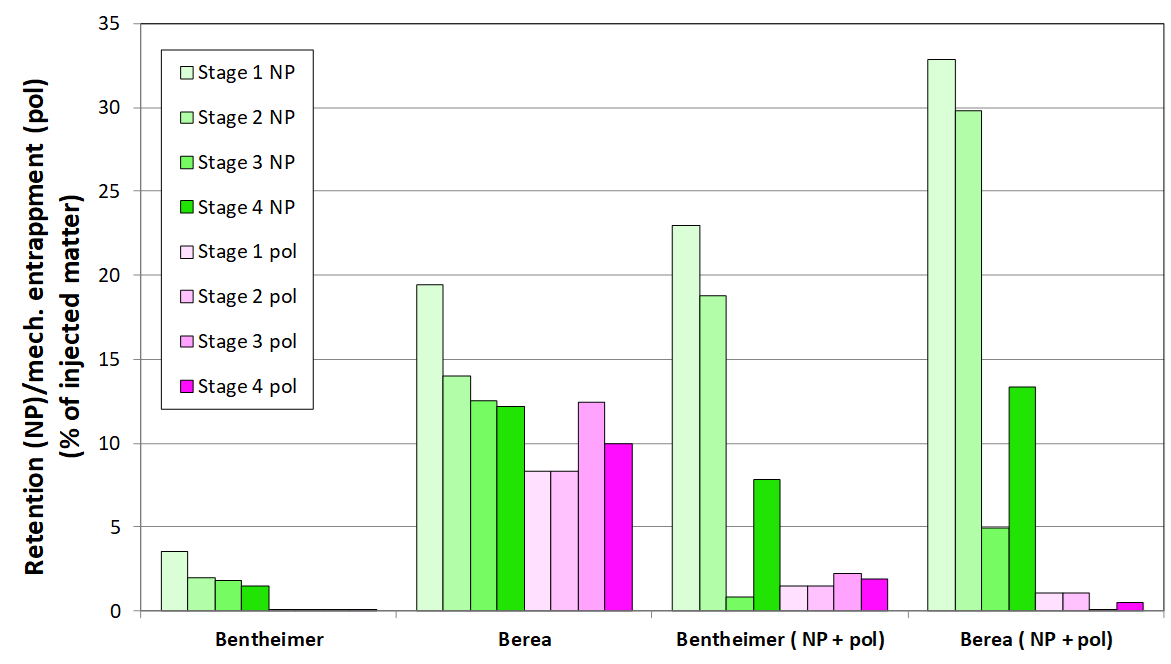
\includegraphics[width=\textwidth]{img/cht/retentionMech.png}
    \caption{Residual resistance factors.}
    \label{cht:retentionMech} % 5.24
\end{figure}

For polymer, the mechanical retention was low in all experiments except for injection of only polymer in Berea sandstone. No errors have been detected in the data processing and ta mechanical retention in the order of 10 \% appears to be real. As already discussed, it is curious that the mechanical retention is close to zero with added nanoparticles. 

The retention of only nanoparticles in Berea is associated with large uncertainty, in the order of ± 10 \% of injected matter (cf. Figure \ref{cht:retentionBer}). The large retention of nanoparticles during injection of the mixtures on stages 1 and 2 can possibly be due to detector response problems. 


\section{ Effect of in situ gelling on water flow}
\subsection{Experiment 1: 7 days of aging}
\index{\textit{in situ} gelling} Figure \ref{cht:gelexp1_1} shows the differential pressures over the core and the viscometer tube during injection of the nanoparticle/polymer solution. Around the 1 PV injection mark, the chemical solution breaks through the core, and shortly after the viscosity of the produced solution is stabilized. The differential pressure over the core increased slowly in the first period of the injection, but started to increase rapidly after approximately 3 PV, indicating clogging of the core.

\begin{figure}[h!]
    \centering
    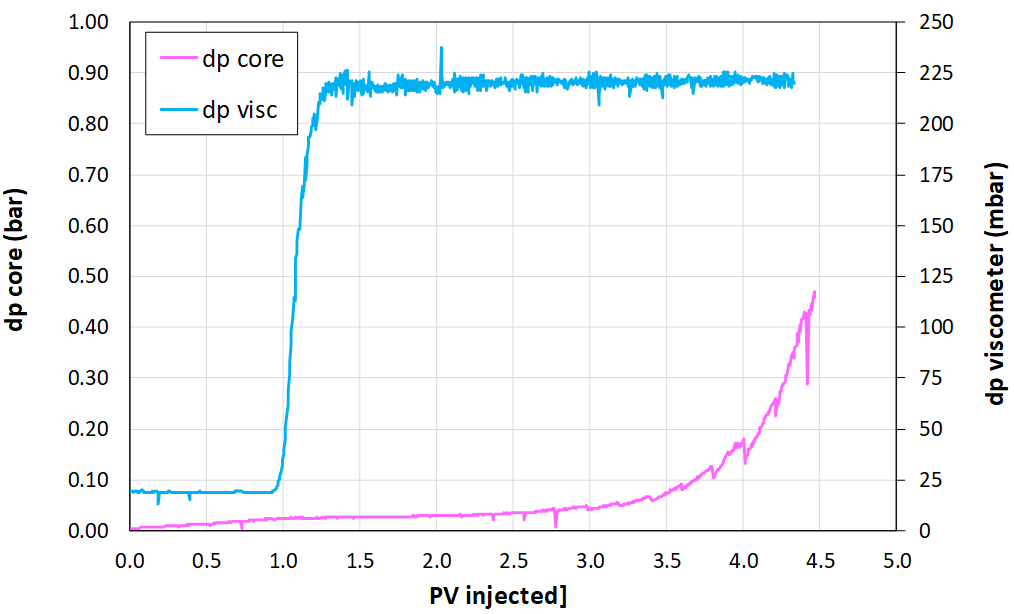
\includegraphics[width=\textwidth]{img/cht/gelexp1_1.png}
    \caption{Experiment 1: Differential pressure over the core and the viscometer tube during injection of the nanoparticle/polymer solution.}
    \label{cht:gelexp1_1} % 5.26
\end{figure}

Figure \ref{cht:gelexp1_2} and Figure \ref{cht:gelexp1_3} show the differential pressures over the core and the viscometer tube during injection of SSW. The differential pressure across the viscometer tube starts to decrease after approximately 0.2 PV and soon approaches the value for SSW. The differential pressure across the core remained almost constant for the first PV SSW injected, but then declined for the next 35 PV before it stabilised at a low value for the rest of the experiment. The water permeability measured at the end of the experiment was 306 mD. Except for two data points the measurement data lays close to the expected straight line as shown in Figure \ref{cht:gelexp1_4}.

\begin{figure}[h!]
    \centering
    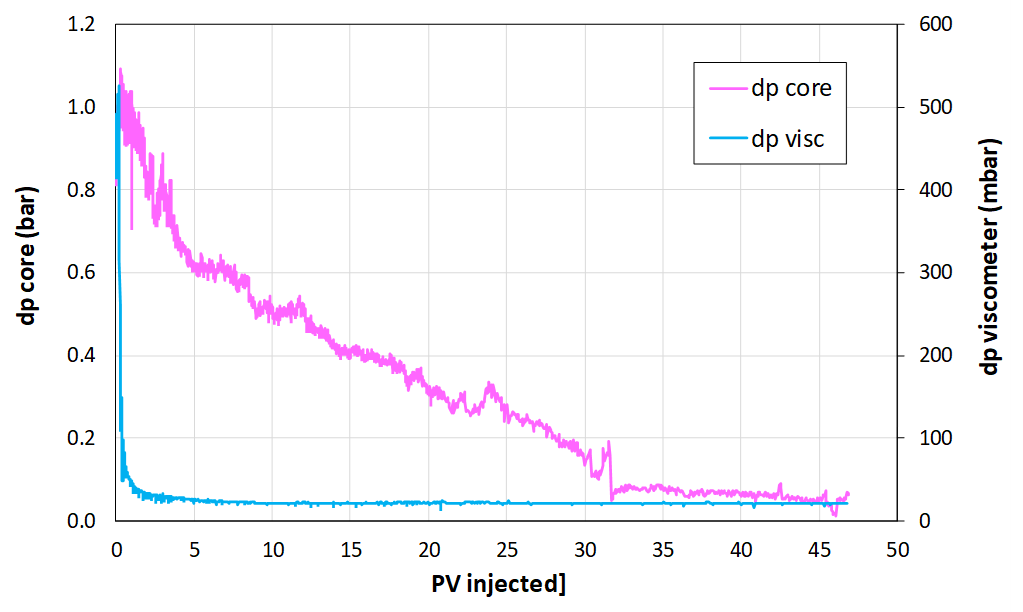
\includegraphics[width=\textwidth]{img/cht/gelexp1_2.png}
    \caption{Experiment 1: Differential pressure over the core and the viscometer tube during injection of SSW into the core aged for 8 days with the nanoparticle/polymer solution.}
    \label{cht:gelexp1_2} % 5.27
\end{figure}

\begin{figure}[h!]
    \centering
    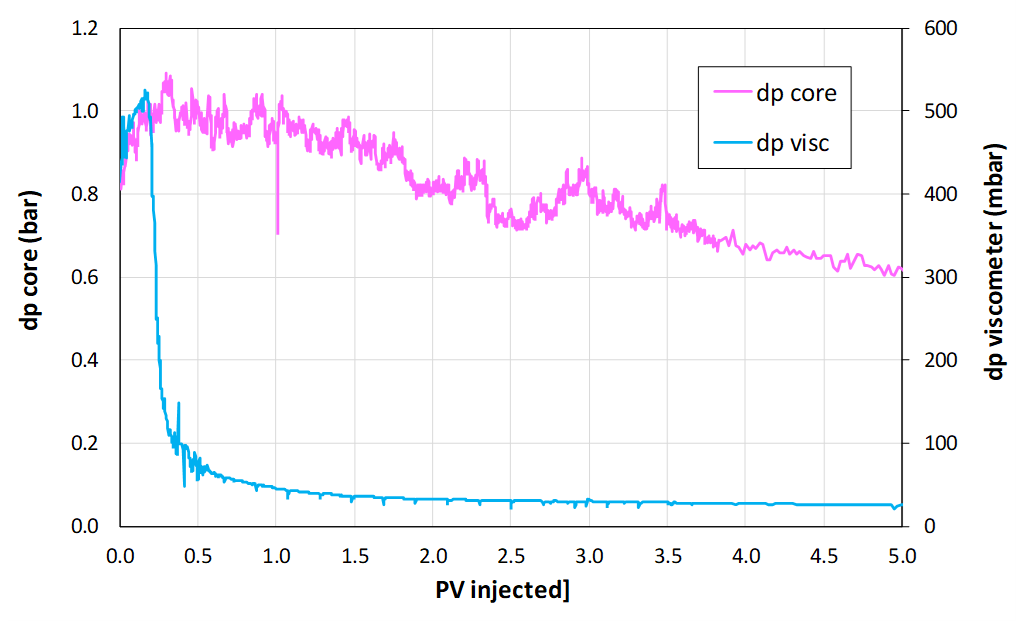
\includegraphics[width=\textwidth]{img/cht/gelexp1_3.png}
    \caption{Experiment 1: (zoomed in on the first 5 PVs) Differential pressure over the core and the viscometer tube during injection of SSW into the core aged for 8 days with the nanoparticle/polymer solution.}
    \label{cht:gelexp1_3} % 5.28
\end{figure}

\begin{figure}[h!]
    \centering
    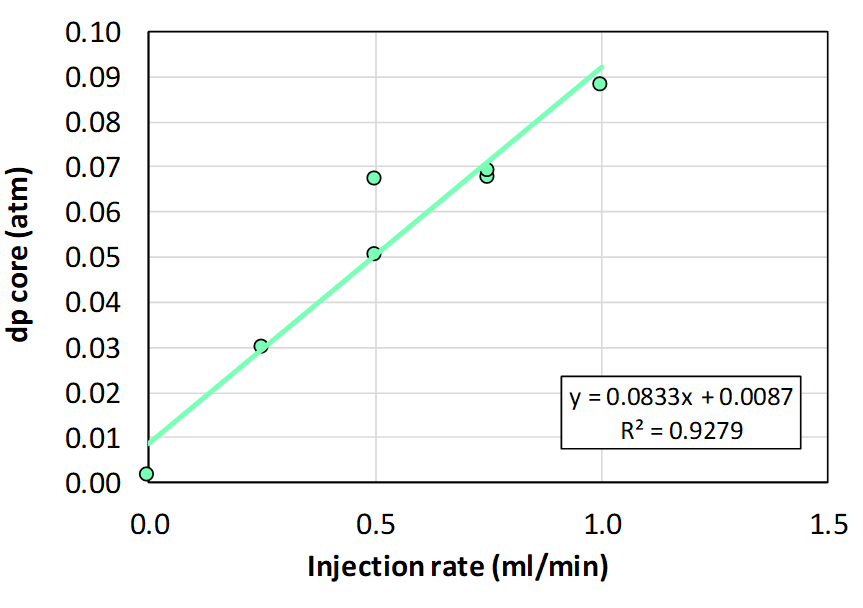
\includegraphics[width=.9\textwidth]{img/cht/gelexp1_4.png}
    \caption{Measured SSW permeability at the end of Experiment 1.}
    \label{cht:gelexp1_4} % 5.29
\end{figure}

\FloatBarrier
\subsection{Experiment 2: 23 days of aging}
Figure \ref{cht:gelexp2_1} shows the differential pressures over the core and the viscometer tube during injection of the nanoparticle/polymer solution. Around the 1 PV injection mark , the chemical solution breaks through the core, and shortly after the viscosity of the produced solution stabilized. The differential pressure over the core increased slowly in the first period of the injection, but started to increase rapidly after approximately 3 PV., indicating clogging of the core. The behaviour was similar to what was observed in the previous experiment (cf. Figure \ref{cht:gelexp1_1}).

\begin{figure}[h!]
    \centering
    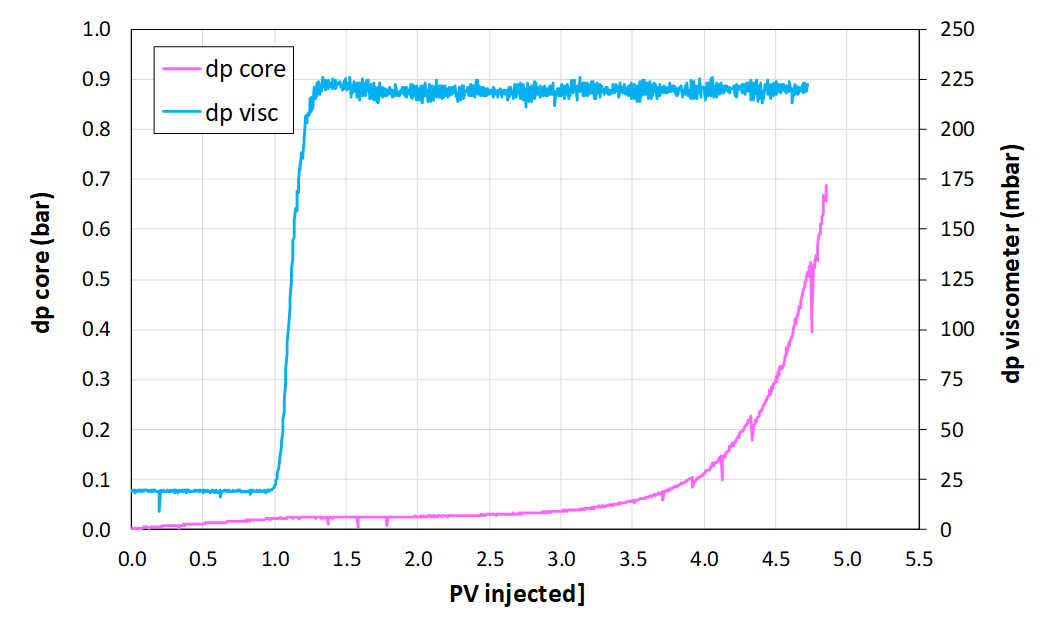
\includegraphics[width=\textwidth]{img/cht/gelexp2_1.png}
    \caption{Experiment 2: Differential pressure over the core and the viscometer tube during injection of the nanoparticle/polymer solution.}
    \label{cht:gelexp2_1} % 5.30
\end{figure}

Figure \ref{cht:gelexp2_2} and Figure \ref{cht:gelexp2_3} show the differential pressures over the core and the viscometer tube during injection of SSW. The differential pressure across the viscometer tube starts to decrease after approximately 0.28 PV and soon approaches the value for SSW. The differential pressure across the core started at 17 bar and fell rapidly to 12 bar and the decreased almost linearly throughout the injection. At the end of the experiment it was 4 bar, significantly higher than the 0.07 bar at a similar stage for the core that had aged for only 7 days (Figure \ref{cht:gelexp1_3}). 

The water permeability measured after 55 PV was only 5 mD. The multi-rate permeability measurements did not give a straight line for the differential pressure vs. flow rate plot (cf. Figure \ref{cht:gelexp2_4} ) which is consistent with the steadily falling differential pressure during the SSW injection. The deviation from the zero rate data point is significant.


\begin{figure}[h!]
    \centering
    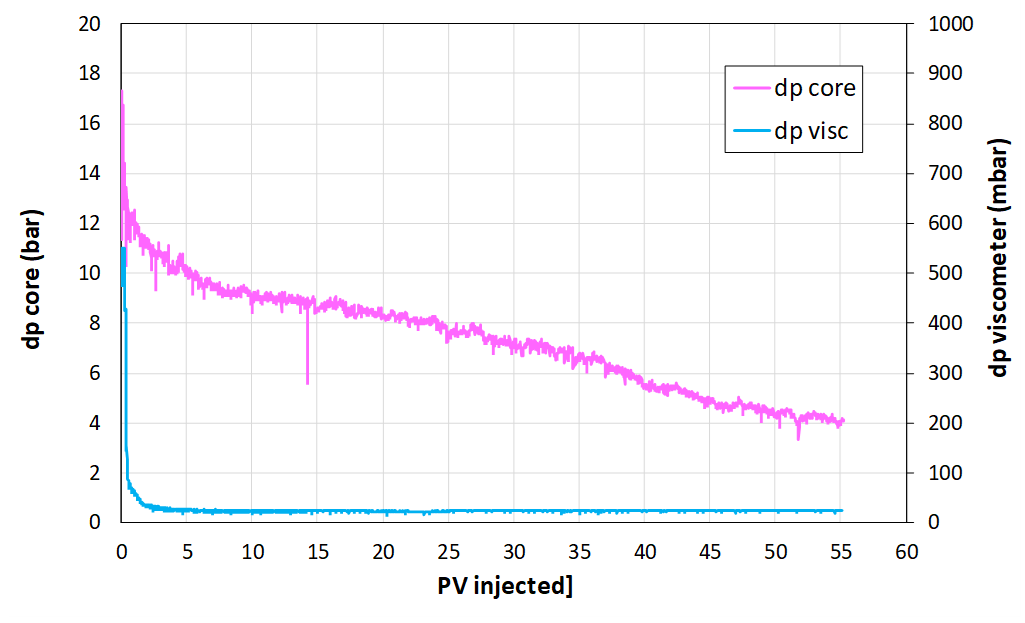
\includegraphics[width=\textwidth]{img/cht/gelexp2_2.png}
    \caption{Experiment 2: Differential pressure over the core and the viscometer tube during injection of SSW into the core aged for 23 days with the nanoparticle/polymer solution.}
    \label{cht:gelexp2_2} % 5.31
\end{figure}

\begin{figure}[h!]
    \centering
    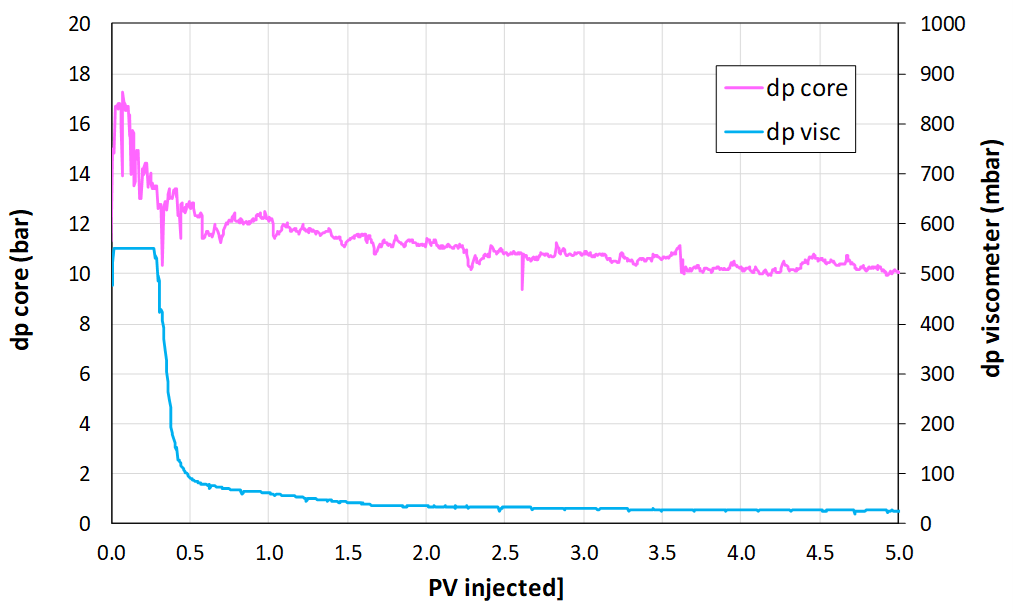
\includegraphics[width=\textwidth]{img/cht/gelexp2_3.png}
    \caption{Experiment 2: (zoomed in on the first 5 PVs)Differential pressure over the core and the viscometer tube during injection of SSW into the core aged for 23 days with the nanoparticle/polymer solution.}
    \label{cht:gelexp2_3} % 5.32
\end{figure}

\begin{figure}[h!]
    \centering
    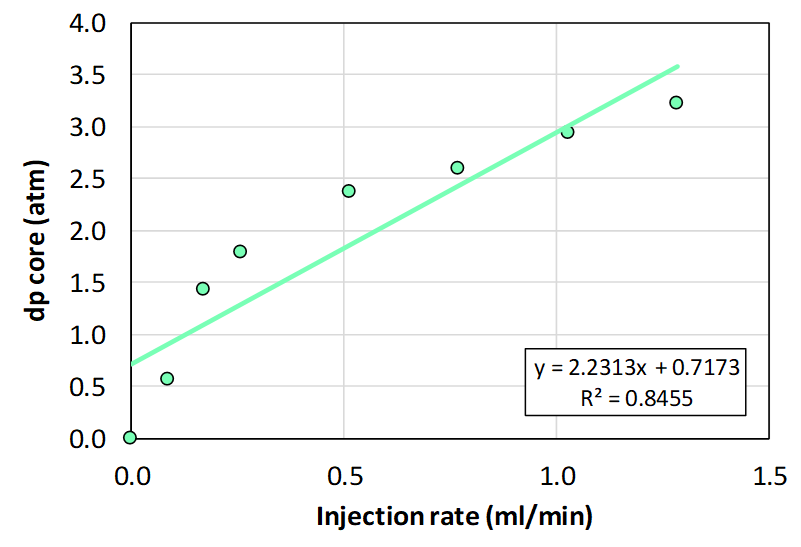
\includegraphics[width=\textwidth]{img/cht/gelexp2_4.png}
    \caption{Measured SSW permeability at the end of Experiment 2.}
    \label{cht:gelexp2_4} % 5.33
\end{figure}

\FloatBarrier
\subsection{Experiment 3: 66 days of aging}

Figure \ref{cht:gelexp3_1} shows the differential pressures over the core and the viscometer tube during injection of the nanoparticle/polymer solution. Around the 1 PV injection mark, the chemical solution breaks through the core, and shortly after, the viscosity of the produced solution is stabilised. The differential pressure over the core increased slowly in the first period of the injection, but started to increase rapidly after approximately 3 PV, indicating clogging of the core. The behaviour was like what was observed in the previous two experiments.



\begin{figure}[h!]
    \centering
    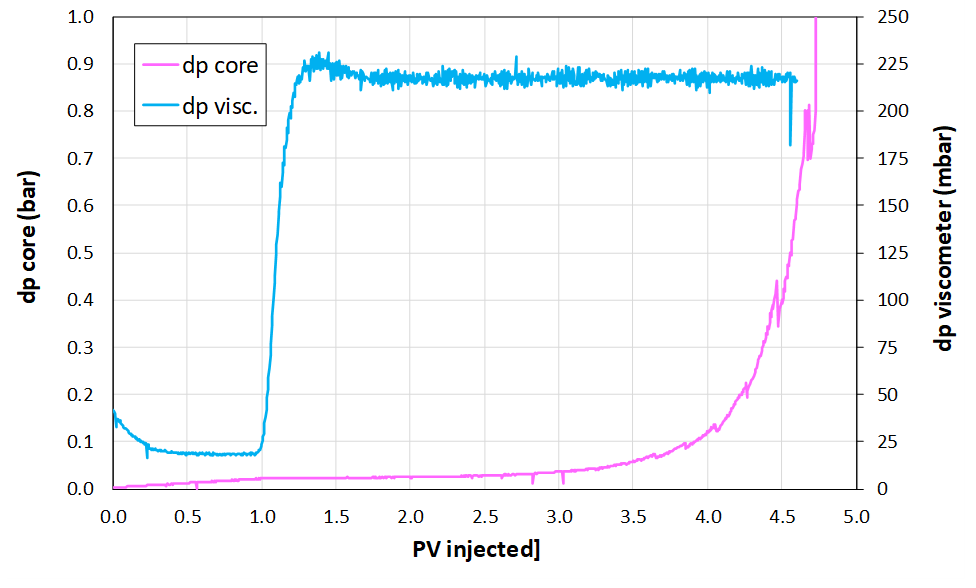
\includegraphics[width=\textwidth]{img/cht/gelexp3_1.png}
    \caption{Experiment 3: Differential pressure over the core and the viscometer tube during injection of the nanoparticle/polymer solution.}
    \label{cht:gelexp3_1} % 5.34
\end{figure}

Figure \ref{cht:gelexp3_2} shows the differential pressures over the core and the viscometer tube during and produced mass as function of time during injection of SSW. Contrary to the previous two experiments, it was not possible to inject SSW at 30 ml/hr at start of the injection. The constant injection rate pump was therefore replaced with a pump restricted by maximum injection pressure (LC-XPD from PYE UNICAM). The maximum injection pressure was set to 27 bar, representing a 135 bar/m pressure gradient across the core. As seen from the figure, little mass was produced from the core during the first 220 hours. After that, the mass production increased during a 10-hour period until the pump reached the set injection rate limit. After approximately 265 hours, the pump was changed to a constant injection rate pump, set to 30 ml/hr.

The differential pressure across the viscometer tube reached values around 20 mbar in the constant injection rate parts of the experiment. This is close to the value measured during the first PV of injection of the nanoparticle/polymer solution (cf. Figure \ref{cht:gelexp3_2}) indicating that only SSW was produced from the core during the experiment.

Figure \ref{cht:gelexp3_3} shows the same measured values as in Figure \ref{cht:gelexp3_2} but plotted against PV injected fluid.

The water permeability measured after 75 PV was only 0.8 mD. The multi-rate permeability measurements gave close to a straight line for the differential pressure vs. flow rate plot but with an offset of more than one atmosphere (Figure \ref{cht:gelexp3_4}).


\begin{figure}[h!]
    \centering
    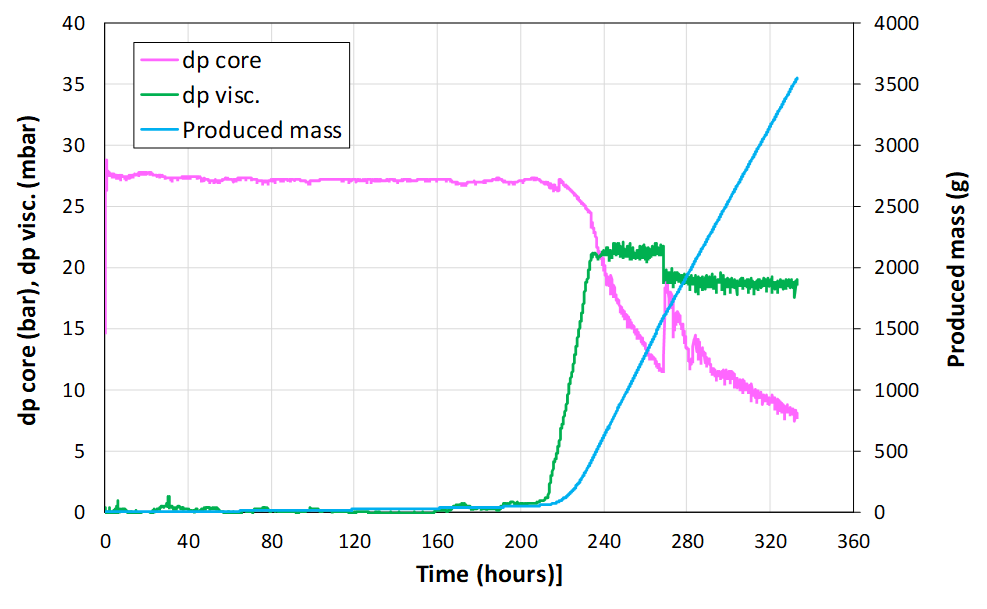
\includegraphics[width=\textwidth]{img/cht/gelexp3_2.png}
    \caption{Experiment 3: Differential pressure over the core and the viscometer tube and produced mass as function of time during injection of SSW into the core aged for 66 days with the nanoparticle/polymer solution.}
    \label{cht:gelexp3_2} % 5.35
\end{figure}

\begin{figure}[h!]
    \centering
    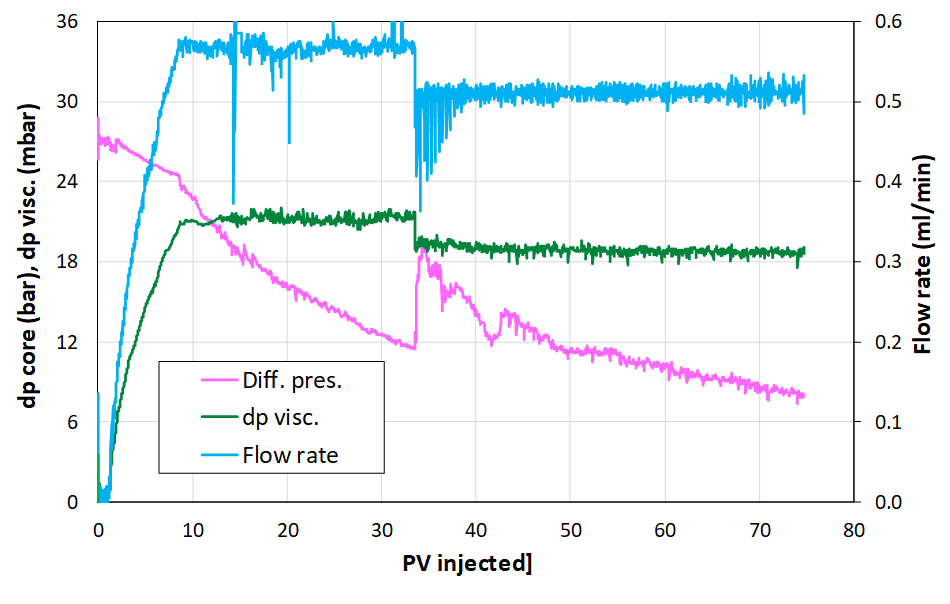
\includegraphics[width=\textwidth]{img/cht/gelexp3_3.png}
    \caption{Experiment 3: (zoomed in) Differential pressure over the core and the viscometer tube during injection of SSW into the core aged for 66 days with the nanoparticle/polymer solution.}
    \label{cht:gelexp3_3} % 5.36
\end{figure}

\begin{figure}[h!]
    \centering
    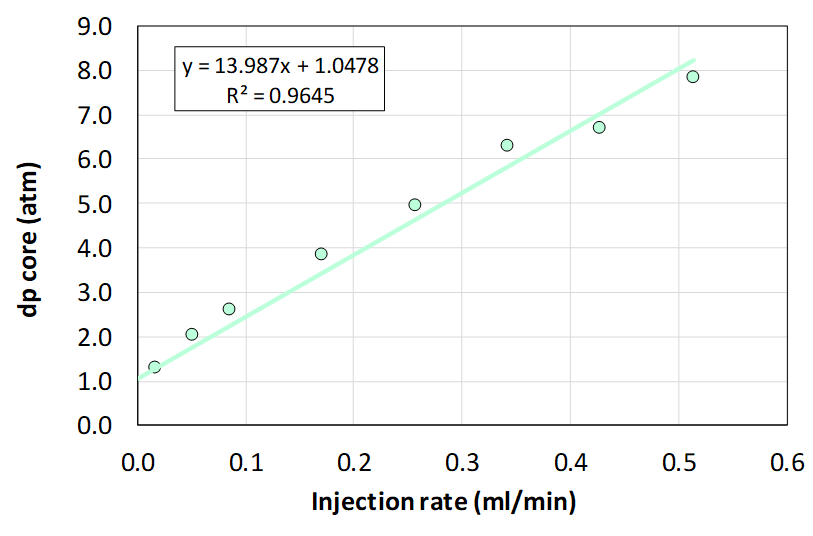
\includegraphics[width=\textwidth]{img/cht/gelexp3_4.png}
    \caption{Measured SSW permeability at the end of Experiment 3.}
    \label{cht:gelexp3_4} % 5.37
\end{figure}

\FloatBarrier
\subsection{Experiment 4: an injectivity test}
\index{injectivity test} As seen in Figure \ref{cht:gelexp1_1}, Figure \ref{cht:gelexp2_1} and Figure \ref{cht:gelexp3_1}, the differential pressures across the cores increased significantly during injection of the identical nanoparticle/polymer solutions. This shows that there is a serious injectivity problem with the fluid system. The three first solutions had been filtered through 8 \micro m membrane filters before injection. Up to 5 filters were used to filter approximately 400 ml solution. For Experiment 3, the dry mass of the filters was determined before and after filtration. The result showed that 0.74 \% of the mass in the solution was lost during the filtration. This indicates that there were particles in the solution, and the presence of these particles may have been the cause of the injectivity problem.

In order to test if another type of pre-treatment of the solution could eliminate the problem, a new solution of nanoparticles and polymer was prepared. This solution was filtered through a 5 cm long 0.5 Darcy Berea sandstone at high rate (500 ml/hr). The differential pressure across the core increased by 5 bar during the filtration, and a 5 bar differential pressure remained during SSW injection with the same rate after the filtration. The collected nanoparticle/polymer solution was turbid before filtration, but clear after the filtration (the same was the case for the solutions filtered through membrane filters).

Figure \ref{cht:gelexp4_1} shows the differential pressure over the core and the viscometer tube during injection of the nanoparticle/polymer solution. The produced fluid appeared analogous to the previous experiments. Also, the differential pressure across the core was similar to the previous experiments in the first phase of the injection. However, in contrast to the previous experiments, where the injections stopped when the differential pressures became excessive, the injection of nanoparticle/polymer solution continued here. As illustrated by the figure, the differential pressure increased to almost 9 bar during the injection, and large fluctuations were seen. It appeared as the core became clogged, but when the differential pressure became high enough, the clogged parts of the core opened before new clogging appeared.

\begin{figure}[h!]
    \centering
    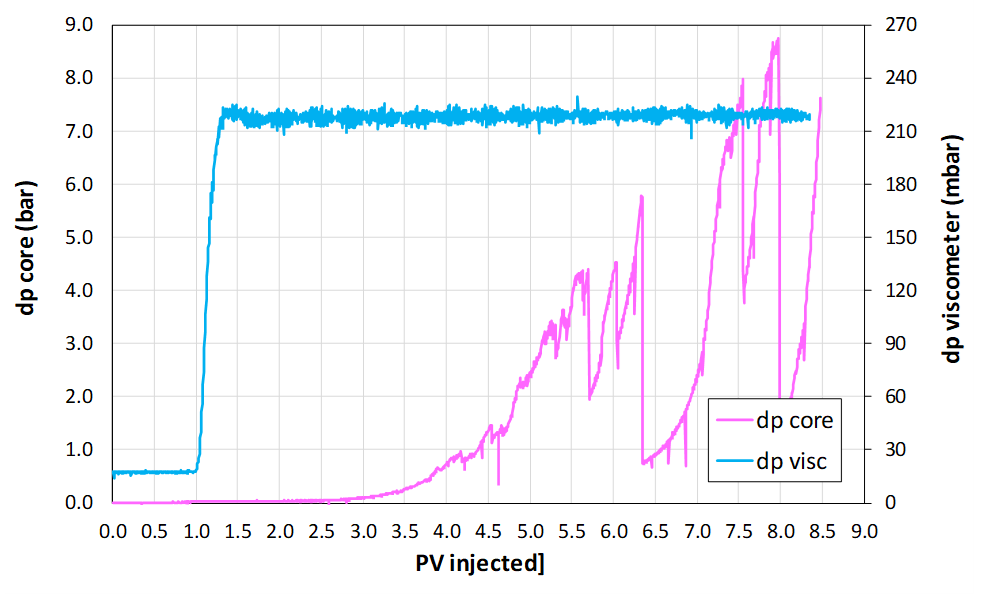
\includegraphics[width=\textwidth]{img/cht/gelexp4_1.png}
    \caption{Experiment 4: Differential pressure over the core and the viscometer tube during injection of the nanoparticle/polymer solution.}
    \label{cht:gelexp4_1} % 5.38
\end{figure}

The results from experiment 4 demonstrated that high rate filtering through a core could not solve the injectivity problem. A natural continuation for addressing the injectivity problem could be to pre-treat the solution through finer porous media than membrane filters or medium permeability cores.

It was speculated that the injectivity problem could be related to poor solubility of the nanoparticle/polymer solution at elevated temperatures. The formation of precipitates at elevated temperatures had not been reported in other work tasks of the project. A simple check was conducted to test if the fast increase in temperature from ambient to 80 ℃ of the injected solution entering the core could have caused instability and precipitation.

Samples of the injected solution were added to three sealed vials and thoroughly purged with argon. One vial was then immersed in a water bath at 80 ℃, one was placed in an oven at 80 ℃ and the last was placed in the oven but immersed in a beaker filled with water.

As a result, the three samples were subjected to fast, medium fast and slow heating. However, no precipitation could be observed in any of the samples.

\FloatBarrier
\subsection{Summary of experiments with in situ gelling}
Table \ref{tab:porPermAge} summarises the initial absolute permeabilities of the cores used in the experiments, the permeabilities measured after the SSW injections and the residual resistance factors, i.e. the ratio between the two permeabilities. The resistance factor determined after 7 days of aging was not much higher than the corresponding factor determined for polymer injection into Bentheimer sandstone, cf. Figure 5.20. As illustrated by the figure, the residual resistance factors increased with longer aging times.
%TAB
\begin{table}
\small
\centering
\caption{Porosities, initial and final permeabilities and residual resistance factor for various aging times.}
\label{tab:porPermAge} % 5.12
\begin{tabular}{c l l l l l } 
\toprule
\textbf{Exp. no.} & \textbf{Porosity} & \textbf{Aging time} & \textbf{Abs. perm.} & \textbf{Residual perm.} & \textbf{RRF} \\ 
 & [fraction] & [days] & [mD] & [mD] & \\
\midrule 
1  & 0.221   &  7     & 2653     & 306      & 8.7    \\
2  & 0.221   & 23     & 2580     & 5.2      & 493      \\ 
3  & 0.221   & 66     & 2706     & 0.008    & 3230   \\ 
\bottomrule
\end{tabular}
\end{table}

The injection phases for the nanoparticle/polymer solution are compared in Figure \ref{cht:gelexp_sum}. As seen the differential pressures across the viscometer tube were similar. In Experiment 3 parts of the bypass line was filled with the nanoparticle/polymer mixture, explaining the initial decline in the viscosity response. 

\begin{figure}[h!]
    \centering
    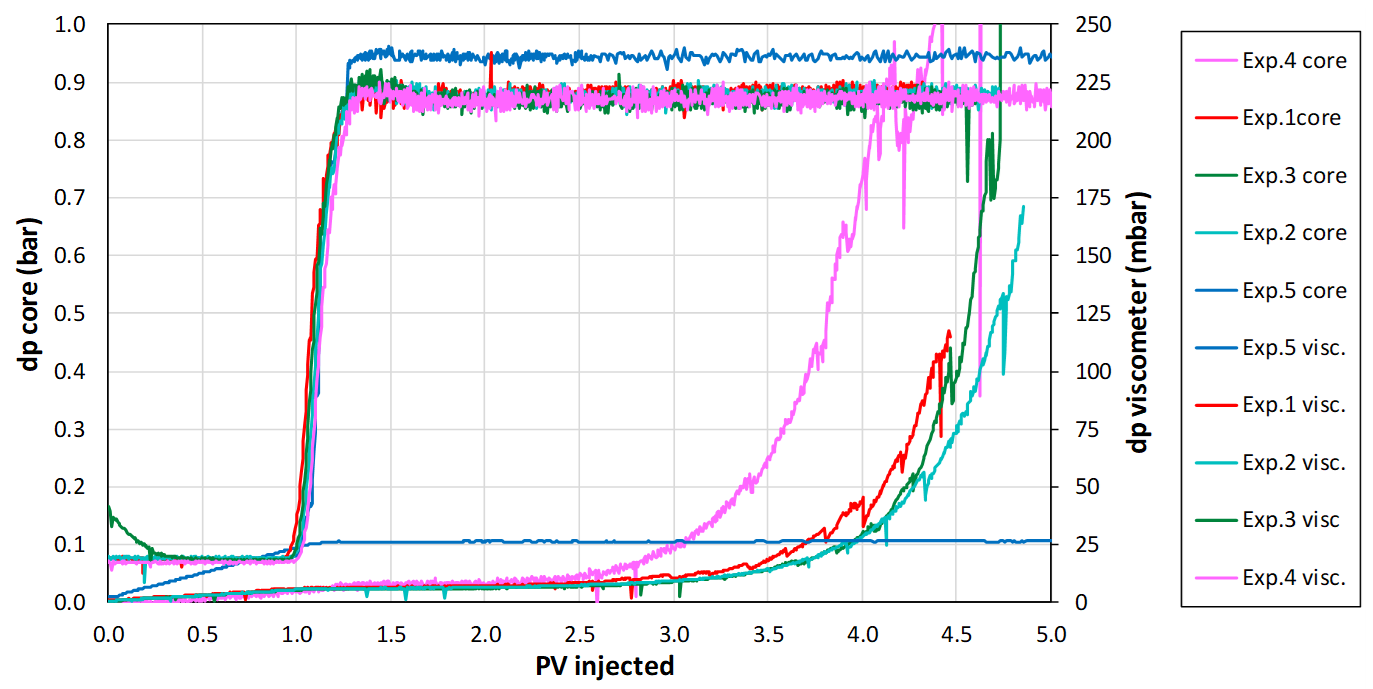
\includegraphics[width=\textwidth]{img/cht/gelexp_sum.png}
    \caption{Comparison of nanoparticle/polymer injection phases.}
    \label{cht:gelexp_sum} % 5.39
\end{figure}
 
The differential pressures over the core developed almost identical for the first 2.5 PVs injected. The rapid increase thereafter, developed in different, but quite similar manners. Filtering through a core apparently gave a less good pre-filtering of the solution compared to filtration through 8 \micro m membrane filters.

If the presence of extended structures/particles in the solution is the cause of the injectivity problem, the use of finer filters, possibly in combination with ultrasonication, could alleviate the problem.

The experiments with in situ gelling has demonstrated that gel is formed in the porous medium. As expected the gel strength increases with increased gelling time. For a gelling time, somewhat longer than 2 months, a strong gel was formed. This gel almost blocked the core with a pressure gradient of 135 bar/m for almost 9 days, but injected SSW could only flow for still large pressure gradients across the core. The residual resistance factor after 75 PV injected was still 3230.

\section{Oil recovery with nanoparticles in injected water}
In measurements done at SINTEF outside the project it was found that addition of FN-nanoparticles could reduce the interfacial tension between brine and crude oil as well as changing the oil-water contact angle on several minerals. It was therefore a good idea to perform core flooding experiments in order to test a possible EOR effect. Two core flooding experiments were conducted where 1 wt.\% FN-PEGMEA-100 141128 was added tom SSW. 1.5 in. Berea sandstone cores were used in the experiments. The experiments were carried out in the setup shown in Figure \ref{fig:experimentalSetup} but the various detecting systems were bypassed. The produced fluids were collected in small samples using a fraction collector (Gilson Model 222) during the first part of the experiments, later larger collection vessels were used. The pump rate was 14 ml/hr. A back pressure of 6 bar was used.

Initial water saturation in the core was established by drop-wise adding 10 g of SSW on the core surface before the core was wrapped in Ni-foil and mounted in the core holder. The following day kerosene (IsoparL) was injected into the core until all air was removed. Oil permeability at initial water saturation was measured and the core holder was heated to process temperature. Basic core data and experimental conditions are summarised in Table 5.13.


\begin{table}
\small
\centering
\caption{Basic core data and some experimental conditions}
\label{tab:coreConditions} % 5.13
\begin{tabular}{c l l l l l l } 
\toprule
\textbf{Experiment no.*} & \textbf{Length} & \textbf{PV} & \textbf{$\boldsymbol{K}_o(\boldsymbol{S}_{wi})$} & \textbf{$\boldsymbol{S}_{wi}$} & \textbf{Temp} & \textbf{Oil}\\ 
 & [cm] & [ml] & [Darcy] & [frac. PV] & \celsius & \\
\midrule 
2  & 0.221   &  7     & 2653     & 306      & 8.7  & IsoparL  \\
3  & 0.221   & 23     & 2580     & 5.2      & 493  & crude    \\ 
\bottomrule
\multicolumn{2}{l}{*\textit{Experiment 1 failed.}}\\
\end{tabular}
\end{table}

\subsection{Experiment 2: water wet system}
SSW injection was performed shortly after the system was equilibrated at process temperature. Figure \ref{cht:prodexp2} shows the production history as oil production and differential pressure vs pore volumes fluid injected. After approximately 35 PV injected SSW, the injection rate was increased in steps up to 499 ml/hr. Then, after 45 PV, the nanoparticle solution was injected at 14 ml/hr, followed by a bump flood with nanoparticle solution at approximately 52 PV injected. Finally, after 63 PV, SSW was again injected at low rate.

\begin{figure}[h!]
    \centering
    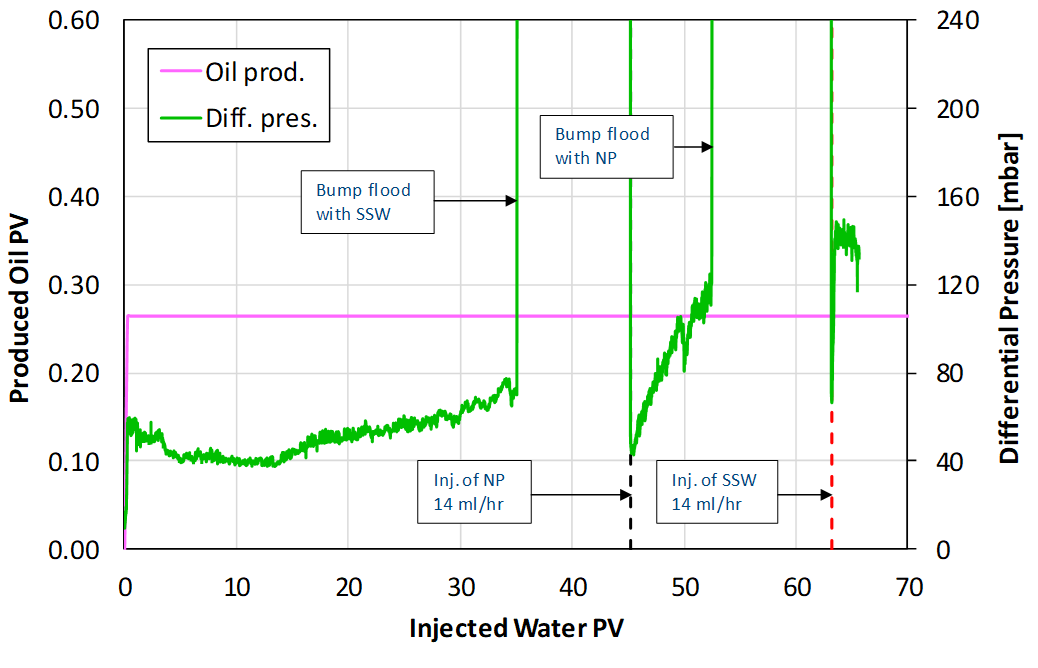
\includegraphics[width=\textwidth]{img/cht/prodexp2.png}
    \caption{Production history for Experiment 2.}
    \label{cht:prodexp2} % 5.40
\end{figure}

Oil was produced as one phase until water breakthrough at 0.264 pore volumes injected. Thereafter there was no quantifiable oil production during the experiment. Only 35.2 \% of the oil originally in place was recovered giving a residual oil saturation as high as 
48.7 \% PV. The poor initial oil recovery was not increased neither by nanoparticles nor the high rate injections (bump floods). The system showed a strong water wet behaviour.

\subsection{Experiment 3: oil wet system}

Experiment 3 was done in essentially the same manner as Experiment 2 with the difference that the core was aged with crude oil for 16 days before water injection started. The viscosity of the crude oil was determined to 1.92 cp at process condition. This value was found by assuming that the permeability measured with kerosene and crude oil the same day were identical. After aging the permeability had decreased to 0.842 Darcy. The density of the crude at process conditions was determined to 0.870 g/ml.

Figure \ref{cht:prodexp3} shows the production history of Experiment 3. The oil production curve exhibits what can be characterised as a typical neutral wet system with high total oil recovery, high recovery at water break through (~0.4 PV) and a significant tail in the oil production. The water permeability at the end of the flood was not very high, i.e. 0.184 Darcy. The relatively high value may have been due to injection of nanoparticles, compare the differential pressures measured at 14 ml/hr injection rate at 35 PV and 61 PV, respectively.

\begin{figure}[h!]
    \centering
    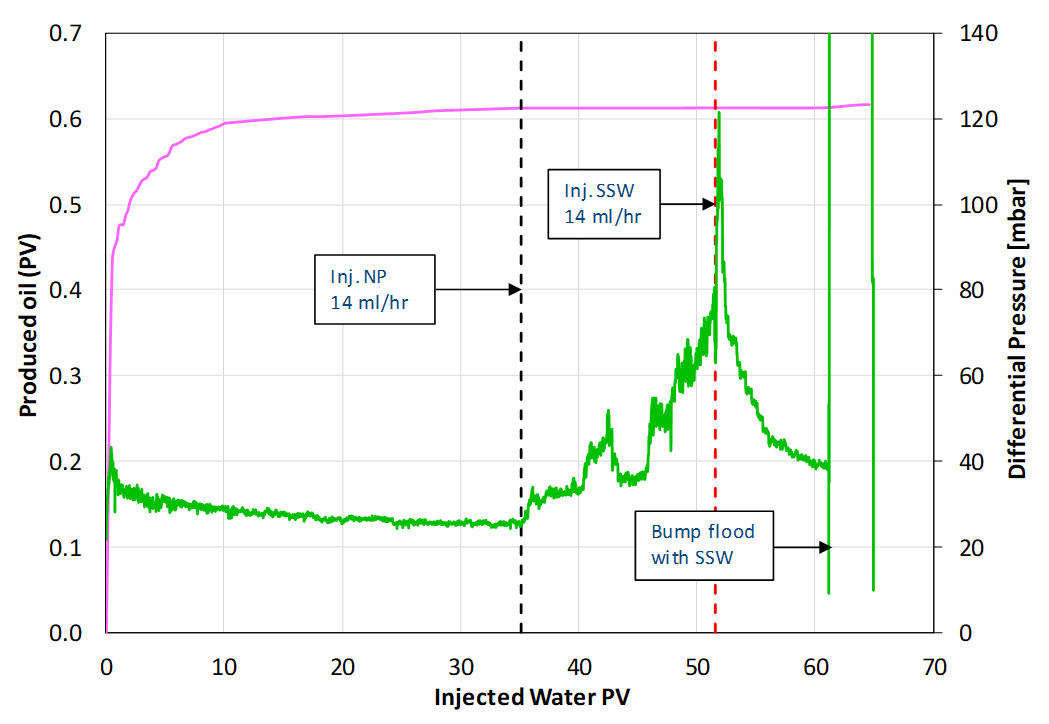
\includegraphics[width=\textwidth]{img/cht/prodexp3.png}
    \caption{Production history for Experiment 3.}
    \label{cht:prodexp3} % 5.41
\end{figure}

As seen in the figure the oil production ceased during the first stage of SSW injection. Injection of nanoparticles did not recover additional oil. A minute amount of oil (0.004 PV) was produced during the bump flood with SSW (4 ml/min) and the subsequent water permeability measurement. At the end of the experiment, the oil residual saturation was 0.136. During the experiment, 81.9 \% of the oil originally in place was recovered.

\subsection{Summary of oil recovery experiments}

The oil recovery experiments demonstrated that the wettability of the rock can have a significant effect on the oil recovery during SSW injection. For the water wet system, the oil recovery was poor, i.e. only 35.2 \% of the original oil in place. The neutral wet system behaved completely differently, as 81.9 \% of the oil originally in place was recovered. The addition of FN-nanoparticles did not affect the recovery in neither of the experiments.




